\let\negmedspace\undefined
\let\negthickspace\undefined
\documentclass[journal,12pt,onecolumn]{article}
\usepackage{cite}
\usepackage{amsmath,amssymb,amsfonts,amsthm}
\usepackage{algorithmic}
\usepackage{graphicx}
\usepackage{textcomp}
\usepackage{xcolor}
\usepackage{txfonts}
\usepackage{listings}
\usepackage{enumitem}
\usepackage{mathtools}
\usepackage{gensymb}
\usepackage{comment}
\usepackage[breaklinks=true]{hyperref}
\usepackage{tkz-euclide} 
\usepackage{listings}
\usepackage{gvv}                                        
%\def\inputGnumericTable{}                                 
\usepackage[latin1]{inputenc}     
\usepackage{xparse}
\usepackage{color}                                            
\usepackage{array}                                            
\usepackage{longtable}                                       
\usepackage{calc}                                             
\usepackage{multirow}
\usepackage{multicol}
\usepackage{hhline}                                           
\usepackage{ifthen}                                           
\usepackage{lscape}
\usepackage{tabularx}
\usepackage{array}
\usepackage{float}
\usepackage{bm}
\newtheorem{theorem}{Theorem}[section]
\newtheorem{problem}{Problem}
\newtheorem{proposition}{Proposition}[section]
\newtheorem{lemma}{Lemma}[section]
\newtheorem{corollary}[theorem]{Corollary}
\newtheorem{example}{Example}[section]
\newtheorem{definition}[problem]{Definition}
\newcommand{\BEQA}{\begin{eqnarray}}
\newcommand{\EEQA}{\end{eqnarray}}
\usepackage{float}
%\newcommand{\define}{\stackrel{\triangle}{=}}
\theoremstyle{remark}
\usepackage{ circuitikz }
%\newtheorem{rem}{Remark}
% Marks the beginning of the document
\begin{document}

\title{CE - 2024}
\author{EE25BTECH11043 - Nishid Khandagre}
\date{}
\maketitle

\renewcommand{\thefigure}{\theenumi}
\renewcommand{\thetable}{\theenumi}

\textbf{SESSION - 1}

\section*{General Aptitude \brak{GA}}
\textbf{Q.1 - Q.5 Carry ONE mark Each}

\begin{enumerate}
    \item If '$\rightarrow$' denotes increasing order of intensity, then the meaning of the words
    \sbrak{\text{simmer $\rightarrow$ seethe $\rightarrow$ smolder}} is analogous to \sbrak{\text{break $\rightarrow$ raze $\rightarrow$ \underline{\hspace{2cm}}}}.
    Which one of the given options is appropriate to fill the blank?

    \hfill{\brak{\text{GATE CE 2024}}}
    \begin{enumerate}
        \item obfuscate
        \item obliterate
        \item fracture
        \item fissure
    \end{enumerate}

    \item In a locality, the houses are numbered in the following way:\\
    The house-numbers on one side of a road are consecutive odd integers starting from 301, while the house-numbers on the other side of the road are consecutive even numbers starting from 302. The total number of houses is the same on both sides of the road.
    If the difference of the sum of the house-numbers between the two sides of the road is 27, then the number of houses on each side of the road is

    \hfill{\brak{\text{GATE CE 2024}}}
    \begin{enumerate}
        \item 27
        \item 52
        \item 54
        \item 26
    \end{enumerate}
    
    \item For positive integers $p$ and $q$, with $\frac{p}{q} \neq 1$, if 
    \begin{align}
    \brak{\frac{p}{q}}^{\frac{p}{q}} = p^{\brak{\frac{p}{q}-1}}
    \end{align} Then,

    \hfill{\brak{\text{GATE CE 2024}}}
    \begin{enumerate}
        \item $q^p = p^q$
        \item $q^p = p^{2q}$
        \item $\sqrt[p]{q} = \sqrt[q]{p}$
        \item $\sqrt[p]{q} = \sqrt[q]{p}$
    \end{enumerate}

    \item Which one of the given options is a possible value of $x$ in the following sequence?
    
    3, 7, 15, $x$, 63, 127, 255

    \hfill{\brak{\text{GATE CE 2024}}}
    \begin{enumerate}
        \item 35
        \item 40
        \item 45
        \item 31
    \end{enumerate}

    \item On a given day, how many times will the second-hand and the minute-hand of a clock cross each other during the clock time 12:05:00 hours to 12:55:00 hours?
    
    \hfill{\brak{\text{GATE CE 2024}}}
    \begin{enumerate}
        \item 51
        \item 49
        \item 50
        \item 55
    \end{enumerate}

\textbf{Q.6 - Q.10 Carry TWO marks Each}

    \item In the given text, the blanks are numbered \brak{i}-\brak{iv}. Select the best match for all the blanks.
    
    From the ancient Athenian arena to the modern Olympic stadiums, athletics \underline{\hspace{2cm}} \brak{i} the potential for a spectacle. The crowd \underline{\hspace{2cm}} \brak{ii} with bated breath as the Olympian artist twists his body, stretching the javelin behind him. Twelve strides in, he begins to cross-step. Six cross-steps \underline{\hspace{2cm}} \brak{iii} in an abrupt stop on his left foot. As his body \underline{\hspace{2cm}} \brak{iv} like a door turning on a hinge, the javelin is launched skyward at a precise angle.

    \hfill{\brak{\text{GATE CE 2024}}}
    \begin{enumerate}
        \item \brak{i} hold \brak{ii} waits \brak{iii} culminates \brak{iv} pivot
        \item \brak{i} holds \brak{ii} wait \brak{iii} culminates \brak{iv} pivot
        \item \brak{i} hold \brak{ii} wait \brak{iii} culminate \brak{iv} pivots
        \item \brak{i} holds \brak{ii} waits \brak{iii} culminate \brak{iv} pivots
    \end{enumerate}

    \item Three distinct sets of indistinguishable twins are to be seated at a circular table that has 8 identical chairs. Unique seating arrangements are defined by the relative positions of the people. How many unique seating arrangements are possible such that each person is sitting next to their twin?

    \hfill{\brak{\text{GATE CE 2024}}}
    \begin{enumerate}
        \item 12
        \item 14
        \item 10
        \item 28
    \end{enumerate}

    \item The chart given below \figref{fig:q8} compares the Installed Capacity \brak{MW} of four power generation technologies, T1, T2, T3, and T4, and their Electricity Generation \brak{MWh} in a time of 1000 hours \brak{h}.
    \begin{figure}[H]
        \centering
        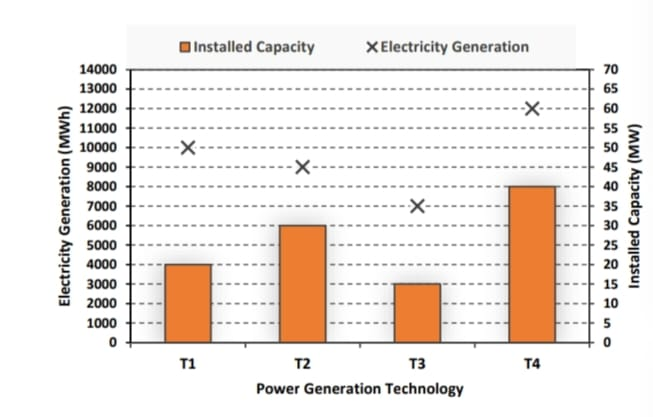
\includegraphics[width=0.7\columnwidth]{figs/1Q8.jpg}
        \caption{}
        \label{fig:q8}
    \end{figure}
    The Capacity Factor of a power generation technology is:
    \begin{align}
    \text{Capacity Factor} = \frac{\text{Electricity Generation (MWh)}}{\text{Installed Capacity (MW)} \times 1000 \text{(h)}}
    \end{align}
    Which one of the given technologies has the highest Capacity Factor?

    \hfill{\brak{\text{GATE CE 2024}}}
    \begin{enumerate}
        \item T1
        \item T2
        \item T3
        \item T4
    \end{enumerate}

    \item In the 4 $\times$ 4 array shown below \figref{fig:q9}, each cell of the first three columns has either a cross \brak{X} or a number, as per the given rule.
    \begin{figure}[H]
        \centering
        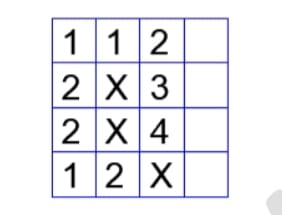
\includegraphics[width=0.25\columnwidth]{figs/1Q9.jpg}
        \caption{}
        \label{fig:q9}
    \end{figure}
    \textbf{Rule:} The number in a cell represents the count of crosses around its immediate neighboring cells \brak{\text{left, right, top, bottom, diagonals}}.
    As per this rule, the \textbf{maximum} number of crosses possible in the empty column is

    \hfill{\brak{\text{GATE CE 2024}}}
    \begin{enumerate}
        \item 0
        \item 1
        \item 2
        \item 3
    \end{enumerate}

    \item During a half-moon phase, the Earth-Moon-Sun form a right triangle. If the Moon-Earth-Sun angle at this half-moon phase is measured to be $89.85\degree$, the ratio of the Earth-Sun and Earth-Moon distances is closest to

    \hfill{\brak{\text{GATE CE 2024}}}
    \begin{enumerate}
        \item 328
        \item 382
        \item 238
        \item 283
    \end{enumerate}

    \item The smallest positive root of the equation
    \begin{align}
    x^5 - 5x^4 - 10x^3 + 50x^2 + 9x - 45 = 0
    \end{align}
    lies in the range

    \hfill{\brak{\text{GATE CE 2024}}}
    \begin{enumerate}
        \item $0 < x \le 2$
        \item $2 < x \le 4$
        \item $6 \le x \le 8$
        \item $10 \le x \le 100$
    \end{enumerate}

    \item The second-order differential equation in an unknown function $u\colon u\brak{x, y}$ is defined as
    \begin{align}
    \frac{\partial^2 u}{\partial x^2} = 2
    \end{align}
    Assuming $g\colon g\brak{x}$, $f\colon f\brak{y}$, and $h\colon h\brak{y}$, the general solution of the above differential equation is

    \hfill{\brak{\text{GATE CE 2024}}}
    \begin{enumerate}
        \item $u = x^2 + f\brak{y} + g\brak{x}$
        \item $u = x^2 + x f\brak{y} + h\brak{y}$
        \item $u = x^2 + x f\brak{y} + g\brak{x}$
        \item $u = x^2 + f\brak{y} + y g\brak{x}$
    \end{enumerate}

    \item The probability that a student passes only in Mathematics is $\frac{1}{3}$. The probability that the student passes only in English is $\frac{4}{9}$. The probability that the student passes in both of these subjects is $\frac{1}{6}$. The probability that the student will pass in at least one of these two subjects is

    \hfill{\brak{\text{GATE CE 2024}}}
    \begin{enumerate}
        \item $\frac{17}{18}$
        \item $\frac{11}{18}$
        \item $\frac{14}{18}$
        \item $\frac{1}{18}$
    \end{enumerate}

    \item The three-dimensional state of stress at a point is given by
    \begin{align}
    \sigma = \myvec{10 & 0 & 0 \\ 0 & 40 & 0 \\ 0 & 0 & 0} \text{MPa.}
    \end{align}
    The maximum shear stress at the point is

    \hfill{\brak{\text{GATE CE 2024}}}
    \begin{enumerate}
        \begin{multicols}{2}
            \item 20 MPa
            \item 15 MPa
            \item 5 MPa
            \item 25 MPa
        \end{multicols}
    \end{enumerate}

    \item Concrete of characteristic strength 30 MPa is required. If 40 specimens of concrete cubes are to be tested, the minimum number of specimens having at least 30 MPa strength should be
    
    \hfill{\brak{\text{GATE CE 2024}}}
    \begin{enumerate}
        \begin{multicols}{2}
            \item 35
            \item 37
            \item 38
            \item 39
        \end{multicols}
    \end{enumerate}

    \item Consider the statements P and Q.
    \begin{itemize}
    \item P: Client's Preliminary Estimate is used for budgeting costs toward the end of planning and design phase.
    \item Q: Client's Detailed Estimate is used for controlling costs during the execution of the project.
    \end{itemize}
    Which one of the following options is CORRECT?

    \hfill{\brak{\text{GATE CE 2024}}}
    \begin{enumerate}
        \item Both P and Q are TRUE
        \item P is TRUE and Q is FALSE
        \item Both P and Q are FALSE
        \item P is FALSE and Q is TRUE
    \end{enumerate}

    \item The following figure \figref{fig:q17} shows the arrangement of formwork for casting a cantilever RC beam.
    \begin{figure}[H]
        \centering
        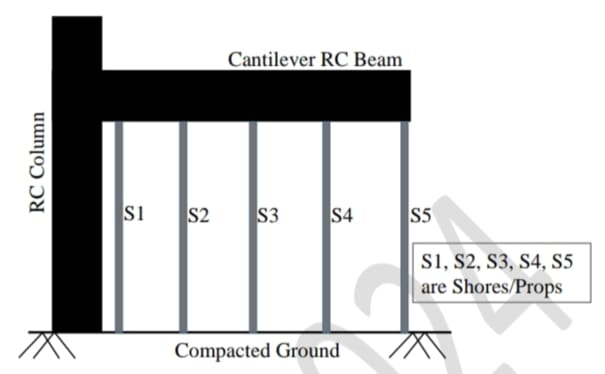
\includegraphics[width=0.7\columnwidth]{figs/1Q17.jpg}
        \caption{}
        \label{fig:q17}
    \end{figure}
    The correct sequence of removing the Shores/Props is

    \hfill{\brak{\text{GATE CE 2024}}}
    \begin{enumerate}
        \item S1$\rightarrow$S2$\rightarrow$S3$\rightarrow$S4$\rightarrow$S5
        \item S5$\rightarrow$S4$\rightarrow$S3$\rightarrow$S2$\rightarrow$S1
        \item S3$\rightarrow$S2$\rightarrow$S4$\rightarrow$S1$\rightarrow$S5
        \item S3$\rightarrow$S4$\rightarrow$S2$\rightarrow$S5$\rightarrow$S1
    \end{enumerate}

    \item A 2 m wide strip footing is founded at a depth of 1.5 m below the ground level in a homogeneous pure clay bed. The clay bed has unit cohesion of 40 kPa. Due to seasonal fluctuations of water table from peak summer to peak monsoon period, the net ultimate bearing capacity of the footing, as per Terzaghi's theory, will
    
    \hfill{\brak{\text{GATE CE 2024}}}
    \begin{enumerate}
        \item remain the same
        \item decrease
        \item increase
        \item become zero
    \end{enumerate}

    \item Consider the statements P and Q.
    \begin{itemize}
    \item P: Soil particles formed by mechanical weathering, and close to their origin are generally subrounded.
    \item Q: Activity of the clay physically signifies its swell potential.
    \end{itemize}
    Which one of the following options is CORRECT?

    \hfill{\brak{\text{GATE CE 2024}}}
    \begin{enumerate}
        \item Both P and Q are TRUE
        \item P is TRUE and Q is FALSE
        \item Both P and Q are FALSE
        \item P is FALSE and Q is TRUE
    \end{enumerate}

    \item The number of degrees of freedom for a natural open channel flow with a mobile bed is
    
    \hfill{\brak{\text{GATE CE 2024}}}
    \begin{enumerate}
        \item 2
        \item 3
        \item 4
        \item 5
    \end{enumerate}

    \item The following table gives various components of Municipal Solid Waste \brak{MSW} and a list of treatment/separation techniques.
    \begin{table}[H]
        \centering
        \begin{tabular}{|l|l|}
            \hline
            \textbf{Component of MSW} & \textbf{Treatment/separation technique} \\
            \hline
            P - Ferrous metals & i - Incineration \\
            Q - Aluminum and copper & ii - Rapid composting \\
            R - Food waste & iii - Eddy current separator \\
            S - Cardboard & iv - Magnetic separator \\
            \hline
        \end{tabular}
        \caption{}
        \label{tab:q21}
    \end{table}
    The CORRECT match is

    \hfill{\brak{\text{GATE CE 2024}}}
    \begin{enumerate}
        \item P-iii, Q-iv, R-i, S-ii
        \item P-iv, Q-iii, R-ii, S-i
        \item P-iii, Q-iv, R-ii, S-i
        \item P-iv, Q-iii, R-i, S-ii
    \end{enumerate}

    \item A car is travelling at a speed of 60 km/hr on a section of a National Highway having a downward gradient of 2\%. The driver of the car suddenly observes a stopped vehicle on the car path at a distance 130 m ahead, and applies brake. If the brake efficiency is 60\%, coefficient of friction is 0.7, driver's reaction time is 2.5 s, and acceleration due to gravity is 9.81 m/s$^2$, the distance \brak{\text{in meters}} required by the driver to bring the car to a safe stop lies in the range
    
    \hfill{\brak{\text{GATE CE 2024}}}
    \begin{enumerate}
        \item 126 to 130
        \item 41 to 45
        \item 33 to 37
        \item 75 to 79
    \end{enumerate}

    \item As per the International Civil Aviation Organization \brak{ICAO}, the basic runway length is increased by x \brak{\%} for every y \brak{m} raise in elevation from the Mean Sea Level \brak{MSL}. The values of x and y, respectively, are
    
    \hfill{\brak{\text{GATE CE 2024}}}
    \begin{enumerate}
        \item 7\% and 300 m
        \item 5\% and 200 m
        \item 4\% and 500 m
        \item 10\% and 1000 m
    \end{enumerate}

    \item Which one of the following statements related to bitumen is FALSE?
    
    \hfill{\brak{\text{GATE CE 2024}}}
    \begin{enumerate}
        \item Kinematic viscosity is a measure of resistance to the flow of molten bitumen under gravity.
        \item Softer grade bitumen possesses higher softening point than hard grade bitumen.
        \item Flash point of bitumen is the lowest temperature at which application of a test flame causes vapours of the bitumen to catch an instant fire in the form of flash under specified test conditions.
        \item Ductility test is carried out on bitumen to test its adhesive property and ability to stretch.
    \end{enumerate}

    \item If the number of sides resulting in a closed traverse is increased from three to four, the sum of the interior angles increases by
    
    \hfill{\brak{\text{GATE CE 2024}}}
    \begin{enumerate}
        \item $90\degree$
        \item $180\degree$
        \item $270\degree$
        \item $360\degree$
    \end{enumerate}

    \item A surveyor observes a zenith angle of $93\degree 00' 00''$ during a theodolite survey. The corresponding vertical angle is
    
    \hfill{\brak{\text{GATE CE 2024}}}
    \begin{enumerate}
        \begin{multicols}{2}
            \item $-03\degree 00' 00''$
            \item $+03\degree 00' 00''$
            \item $-87\degree 00' 00''$
            \item $+87\degree 00' 00''$
        \end{multicols}
    \end{enumerate}

    \item Among the following statements relating the fundamental lines of a transit theodolite, which one is CORRECT?
    
    \hfill{\brak{\text{GATE CE 2024}}}
    \begin{enumerate}
        \item The line of collimation must be perpendicular to the horizontal axis at its intersection with the vertical axis.
        \item The axis of altitude level must be perpendicular to the line of collimation.
        \item The axis of plate level must lie in a plane parallel to the vertical axis.
        \item The Vernier of vertical circle must read zero when the line of collimation is vertical.
    \end{enumerate}

    \item For the following partial differential equation,
    \begin{align}
    x \frac{\partial^2 f}{\partial x^2} + y \frac{\partial^2 f}{\partial y^2} = \frac{x^2 + y^2}{2}
    \end{align}
    which of the following option\brak{s} is/are CORRECT?
    
    \hfill{\brak{\text{GATE CE 2024}}}
    \begin{enumerate}
        \item elliptic for $x > 0$ and $y > 0$
        \item parabolic for $x > 0$ and $y > 0$
        \item elliptic for $x = 0$ and $y > 0$
        \item hyperbolic for $x < 0$ and $y > 0$
    \end{enumerate}

    \item The elements that DO NOT increase the strength of structural steel are
    
    \hfill{\brak{\text{GATE CE 2024}}}
    \begin{enumerate}
        \begin{multicols}{2}
            \item Carbon
            \item Manganese
            \item Sulphur
            \item Chlorine
        \end{multicols}
    \end{enumerate}

    \item Consider a balanced doubly-reinforced concrete section. If the material and other sectional properties remain unchanged, for which of the following cases will the section becomes under-reinforced?
    
    \hfill{\brak{\text{GATE CE 2024}}}
    \begin{enumerate}
        \item Area of tension reinforcement is increased.
        \item Area of compression reinforcement is increased.
        \item Area of tension reinforcement is decreased.
        \item Area of compression reinforcement is decreased.
    \end{enumerate}

    \item The primary air pollutant\brak{s} is/are
    
    \hfill{\brak{\text{GATE CE 2024}}}
    \begin{enumerate}
        \begin{multicols}{2}
            \item Sulphur dioxide
            \item Lead
            \item Ozone
            \item Sulphuric acid
        \end{multicols}
    \end{enumerate}

    \item Consider the data of $f\brak{x}$ given in the table.
    \begin{table}[H]
        \centering
        \begin{tabular}{|c|c|c|c|}
            \hline
            $i$ & 0 & 1 & 2 \\
            \hline
            $x_i$ & 1 & 2 & 3 \\
            \hline
            $f\brak{x_i}$ & 0 & 0.3010 & 0.4771 \\
            \hline
        \end{tabular}
        \caption{}
        \label{tab:q32}
    \end{table}
    The value of $f\brak{1.5}$ estimated using second-order Newton's interpolation formula is \underline{\hspace{2cm}} \brak{\text{rounded off to 2 decimal places}}.
    
    \hfill{\brak{\text{GATE CE 2024}}}

    \item The plane frame shown in the figure \figref{fig:q33} has fixed support at joint A, hinge support at joint F, and roller support at joint I. In the figure, A to I indicate joints of the frame.
    \begin{figure}[H]
        \centering
        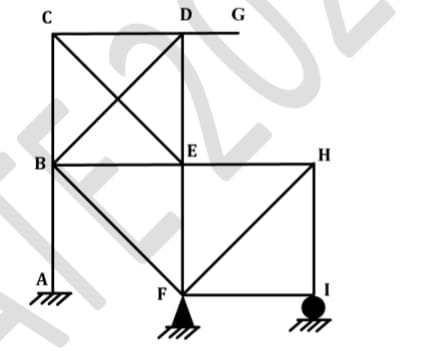
\includegraphics[width=0.7\columnwidth]{figs/1Q33.jpg}
        \caption{}
        \label{fig:q33}
    \end{figure}
    If the axial deformations are neglected, the degree of kinematic indeterminacy is \underline{\hspace{2cm}} \brak{\text{in integer}}.
    
    \hfill{\brak{\text{GATE CE 2024}}}

    \item An embankment is constructed with soil by maintaining the degree of saturation as 75\% during compaction. The specific gravity of soil is 2.68 and the moisture content is 17\% during compaction. Consider the unit weight of water as 10 kN/m$^3$. The dry unit weight \brak{\text{in kN/m$^3$}} of the compacted soil is \underline{\hspace{2cm}} \brak{\text{rounded off to 2 decimal places}}.
    
    \hfill{\brak{\text{GATE CE 2024}}}

    \item A 30 cm diameter well fully penetrates an unconfined aquifer of saturated thickness 20 m with hydraulic conductivity of 10 m/day. Under the steady pumping rate for a long time, the drawdowns in two observation wells located at 10 m and 100 m from the pumping well are 5 m and 1 m, respectively. The corresponding pumping rate \brak{\text{in m$^3$/day}} from the well is \underline{\hspace{2cm}} \brak{\text{rounded off to 2 decimal places}}.
    
    \hfill{\brak{\text{GATE CE 2024}}}

    \textbf{Q.36 - Q.65 Carry TWO marks Each}
    \item What are the eigenvalues of the matrix $\myvec{2 & 1 & 1 \\ 1 & 4 & 1 \\ 1 & 1 & 2}$?
    
    \hfill{\brak{\text{GATE CE 2024}}}
    \begin{enumerate}
        \begin{multicols}{2}
            \item 1, 2, 5
            \item 1, 3, 4
            \item -5, 1, 2
            \item -5, -1, 2
        \end{multicols}
    \end{enumerate}

    \item A vector field $\vec{p}$ and a scalar field $r$ are given by
    \begin{align}
        \vec{p} &= \brak{2x^2 - 3xy + z^2}\hat{i} + \brak{2y^2 - 3yz + x^2}\hat{j} + \brak{2z^2 - 3xz + x^2}\hat{k} \\
        r &= 6x^2 + 4y^2 - z^2 - 9xyz - 2xy + 3xz - yz
    \end{align}
    Consider the statements P and Q. \\
    P: Curl of the gradient of the scalar field $r$ is a null vector. \\
    Q: Divergence of curl of the vector field $\vec{p}$ is zero. \\
    Which one of the following options is CORRECT?
    
    \hfill{\brak{\text{GATE CE 2024}}}
    \begin{enumerate}
        \item Both P and Q are FALSE
        \item P is TRUE and Q is FALSE
        \item P is FALSE and Q is TRUE
        \item Both P and Q are TRUE
    \end{enumerate}
    
    \item Find the correct match between the plane stress states and the Mohr's circles.
    \begin{enumerate}
        \item \begin{figure}[H]
        \centering
        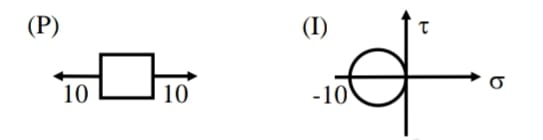
\includegraphics[width=0.7\columnwidth]{figs/1Q38a.jpg}
        \caption{}
        \label{fig:q39}
    \end{figure}
    \item \begin{figure}[H]
        \centering
        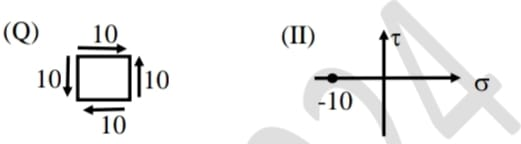
\includegraphics[width=0.7\columnwidth]{figs/1Q38b.jpg}
        \caption{}
        \label{fig:q39}
    \end{figure}
    \item \begin{figure}[H]
        \centering
        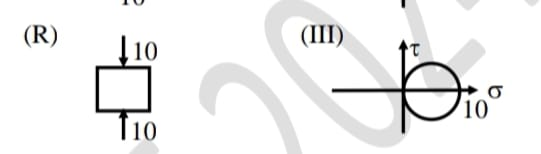
\includegraphics[width=0.7\columnwidth]{figs/1Q38c.jpg}
        \caption{}
        \label{fig:q39}
    \end{figure}
    \item \begin{figure}[H]
        \centering
        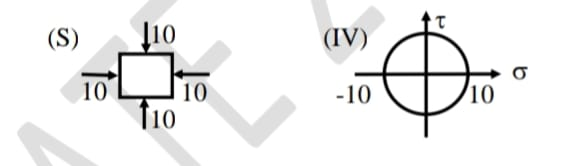
\includegraphics[width=0.7\columnwidth]{figs/1Q38d.jpg}
        \caption{}
        \label{fig:q39}
    \end{figure}    
    \end{enumerate}
    
    \hfill{\brak{\text{GATE CE 2024}}}
    \begin{enumerate}
        \item \brak{P}-\brak{III}; \brak{Q}-\brak{IV}; \brak{R}-\brak{I}; \brak{S}-\brak{II}
        \item \brak{P}-\brak{III}; \brak{Q}-\brak{II}; \brak{R}-\brak{I}; \brak{S}-\brak{IV}
        \item \brak{P}-\brak{I}; \brak{Q}-\brak{IV}; \brak{R}-\brak{III}; \brak{S}-\brak{II}
        \item \brak{P}-\brak{I}; \brak{Q}-\brak{II}; \brak{R}-\brak{III}; \brak{S}-\brak{IV}
    \end{enumerate}
    
    \item The beam shown in the figure \figref{fig:q39} is subjected to a uniformly distributed downward load of intensity $q$ between supports A and B.
    \begin{figure}[H]
        \centering
        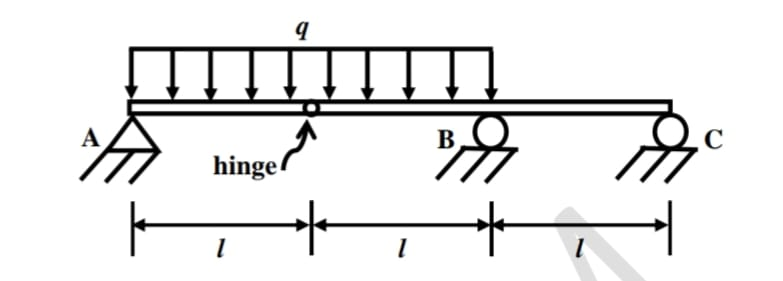
\includegraphics[width=0.7\columnwidth]{figs/1Q39.jpg}
        \caption{}
        \label{fig:q39}
    \end{figure}
    Considering the upward reactions as positive, the support reactions are
    
    \hfill{\brak{\text{GATE CE 2024}}}
    \begin{enumerate}
        \item $R_A = \frac{ql}{2}; R_B = \frac{5ql}{2}; R_C = -ql$
        \item $R_A = -ql; R_B = \frac{5ql}{2}; R_C = -\frac{ql}{2}$
        \item $R_A = -\frac{ql}{2}; R_B = \frac{5ql}{2}; R_C = 0$
        \item $R_A = \frac{ql}{2}; R_B = ql; R_C = \frac{ql}{2}$
    \end{enumerate}
    
    \item A homogeneous shaft PQR with fixed supports at both ends is subjected to a torsional moment T at point Q, as shown in the figure \figref{fig:q40}. The polar moments of inertia of the portions PQ and QR of the shaft with circular cross-sections are $J_1$ and $J_2$, respectively. The torsional moment reactions at the supports P and R are $T_P$ and $T_R$, respectively.
    \begin{figure}[H]
        \centering
        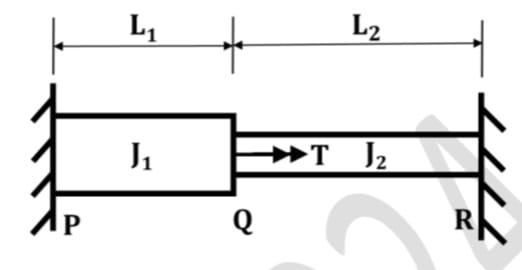
\includegraphics[width=0.7\columnwidth]{figs/1Q40.jpg}
        \caption{}
        \label{fig:q40}
    \end{figure}
    If $T_P/T_R = 4$ and $J_1/J_2 = 2$, the ratio of the lengths $L_1/L_2$ is
    
    \hfill{\brak{\text{GATE CE 2024}}}
    \begin{enumerate}
        \begin{multicols}{2}
            \item 0.50
            \item 0.25
            \item 4.00
            \item 2.00
        \end{multicols}
    \end{enumerate}
    
    \item A vertical smooth rigid retaining wall is supporting horizontal ground with dry cohesionless backfill having a friction angle of $30\degree$. The inclinations of failure planes with respect to the major principal plane for Rankine's active and passive earth pressure conditions, respectively, are
    
    \hfill{\brak{\text{GATE CE 2024}}}
    \begin{enumerate}
        \begin{multicols}{2}
            \item $30\degree$ and $30\degree$
            \item $60\degree$ and $60\degree$
            \item $30\degree$ and $60\degree$
            \item $60\degree$ and $30\degree$
        \end{multicols}
    \end{enumerate}
    
    \item A flow velocity field $\vec{V}: \vec{V}\brak{x, y}$ for a fluid is represented by
    \begin{align}
    \vec{V} = 3\hat{i} + \brak{5x}\hat{j}
    \end{align}
    In the context of the fluid and the flow, which one of the following statements is CORRECT?
    
    \hfill{\brak{\text{GATE CE 2024}}}
    \begin{enumerate}
        \item The fluid is incompressible and the flow is rotational.
        \item The fluid is incompressible and the flow is irrotational.
        \item The fluid is compressible and the flow is rotational.
        \item The fluid is compressible and the flow is irrotational.
    \end{enumerate}
    
    \item For assessing the compliance with the emissions standards of incineration plants, a correction needs to be applied to the measured concentrations of air pollutants. The emission standard \brak{\text{based on 11\% Oxygen}} for HCl is 50 mg/Nm$^3$ and the measured concentrations of HCl and Oxygen in flue gas are 42 mg/Nm$^3$ and 13\%, respectively.
    
    Assuming 21\% Oxygen in air, the CORRECT statement is:
    
    \hfill{\brak{\text{GATE CE 2024}}}
    \begin{enumerate}
        \item No compliance, as the corrected HCl emission is greater than the emission standard.
        \item Compliance is there, as the corrected HCl emission is lesser than the emission standard.
        \item Compliance is there, as there is no need to apply the correction since Oxygen is greater than 11\% and HCl emission is lesser than the emission standard.
        \item No compliance, as the Oxygen is greater than 11\% in the flue gas.
    \end{enumerate}
    
    \item The free mean speed is 60 km/hr on a given road. The average space headway at jam density on this road is 8 m. For a linear speed-density relationship, the maximum flow \brak{\text{in veh/hr/lane}} expected on the road is
    
    \hfill{\brak{\text{GATE CE 2024}}}
    \begin{enumerate}
        \begin{multicols}{2}
            \item 1875
            \item 938
            \item 2075
            \item 1038
        \end{multicols}
    \end{enumerate}
    
    \item A map is prepared with a scale of 1:1000 and a contour interval of 1 m. If the distance between two adjacent contours on the map is 10 mm, the slope of the ground between the adjacent contours is
    
    \hfill{\brak{\text{GATE CE 2024}}}
    \begin{enumerate}
        \begin{multicols}{2}
            \item 30\%
            \item 10\%
            \item 35\%
            \item 40\%
        \end{multicols}
    \end{enumerate}
    
    \item Which of the following statement\brak{s} is/are CORRECT?
    
    \hfill{\brak{\text{GATE CE 2024}}}
    \begin{enumerate}
        \item Swell potential of soil decreases with an increase in the shrinkage limit.
        \item Both loose and dense sands with different initial void ratios can attain similar void ratio at large strain during shearing.
        \item Among the several corrections to be applied to the SPT-N value, the dilatancy correction is applied before all other corrections.
        \item In electrical resistivity tomography, the depth of current penetration is half of the spacing between the electrodes.
    \end{enumerate}
    
    \item The return period of a large earthquake for a given region is 200 years. Assuming that earthquake occurrence follows Poisson's distribution, the probability that it will be exceeded at least once in 50 years is \underline{\hspace{2cm}} \% \brak{\text{rounded off to the nearest integer}}.
    
    \hfill{\brak{\text{GATE CE 2024}}}
    
    \item A 2 m $\times$ 2 m tank of 3 m height has inflow, outflow and stirring mechanisms. Initially, the tank was half-filled with fresh water. At $t = 0$, an inflow of a salt solution of concentration 5 g/m$^3$ at the rate of 2 litre/s and an outflow of the well stirred mixture at the rate of 1 litre/s are initiated. This process can be modelled using the following differential equation:
    \begin{align}
    \frac{dm}{dt} + \frac{m}{6000 + t} = 0.01
    \end{align}
    where $m$ is the mass \brak{grams} of the salt at time $t$ \brak{seconds}. The mass of the salt \brak{\text{in grams}} in the tank at 75\% of its capacity is \underline{\hspace{2cm}} \brak{\text{rounded off to 2 decimal places}}.
    
    \hfill{\brak{\text{GATE CE 2024}}}
    
    \item The plane truss shown in the figure \figref{fig:q49} has 13 joints and 22 members. The truss is made of a homogeneous, prismatic, linearly elastic material. All members have identical axial rigidity. A to M indicate the joints of the truss. The truss has pin supports at joints A and L and roller support at joint K. The truss is subjected to a 10 kN vertically downward force at joint H and a 10 kN horizontal force in the rightward direction at joint B as shown.
    \begin{figure}[H]
        \centering
        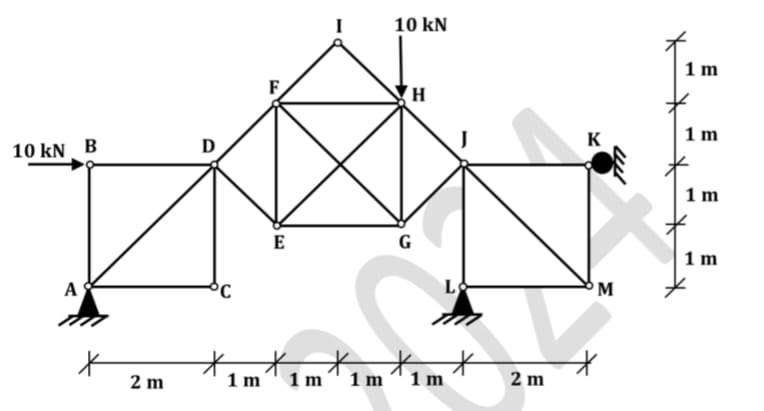
\includegraphics[width=0.7\columnwidth]{figs/1Q49.jpg}
        \caption{}
        \label{fig:q49}
    \end{figure}
    The magnitude of the reaction \brak{\text{in kN}} at the pin support L is \underline{\hspace{2cm}} \brak{\text{rounded off to 1 decimal place}}.
    
    \hfill{\brak{\text{GATE CE 2024}}}
    
    \item An inverted T-shaped concrete beam \brak{B1} in the figure \figref{fig:q50}, with centroidal axis X - X, is subjected to an effective prestressing force of 1000 kN acting at the bottom kern point of the beam cross-section. Also consider an identical concrete beam \brak{B2} with the same grade of concrete but without any prestressing force.
    \begin{figure}[H]
        \centering
        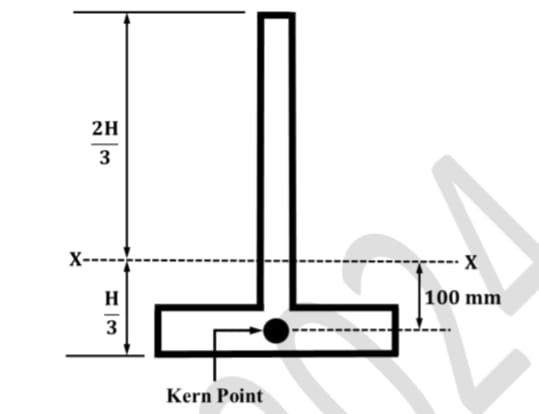
\includegraphics[width=0.7\columnwidth]{figs/1Q50.jpg}
        \caption{}
        \label{fig:q50}
    \end{figure}
    The additional cracking moment \brak{\text{in kN.m}} that can be carried by beam $B1$ in comparison to beam $B2$ is \underline{\hspace{2cm}} \brak{\text{rounded off to the nearest integer}}.
    
    \hfill{\brak{\text{GATE CE 2024}}}
    
    \item The initial cost of an equipment is Rs. 1,00,000. Its salvage value at the end of accounting life of 5 years is Rs. 10,000. The difference in depreciation \brak{\text{in Rs.}} computed using 'double-declining balance method' and 'straight line method' of depreciation in Year-2 is \underline{\hspace{2cm}} \brak{\text{in positive integer}}.
    
    \hfill{\brak{\text{GATE CE 2024}}}
    
    \item A slab panel with an effective depth of 250 mm is reinforced with 0.2\% main reinforcement using 8 mm diameter steel bars. The uniform center-to-center spacing \brak{\text{in mm}} at which the 8 mm diameter bars are placed in the slab panel is \underline{\hspace{2cm}} \brak{\text{rounded off to the nearest integer}}.
    
    \hfill{\brak{\text{GATE CE 2024}}}
    
    \item The total primary consolidation settlement \brak{S_c} of a building constructed on a 10 m thick saturated clay layer is estimated to be 50 mm. After 300 days of the construction of the building, primary consolidation settlement was reported as 10 mm. The additional time \brak{\text{in days}} required to achieve 50\% of S$_c$ will be \underline{\hspace{2cm}} \brak{\text{rounded off to the nearest integer}}.
    
    \hfill{\brak{\text{GATE CE 2024}}}
    
    \item An infinite slope is made up of cohesionless soil with seepage parallel to and up to the sloping surface. The angle of slope is $30\degree$ with respect to horizontal ground surface. The unit weights of the saturated soil and water are 20 kN/m$^3$ and 10 kN/m$^3$, respectively. The minimum angle of shearing resistance of the soil \brak{\text{in degrees}} for the critically stable condition of the slope is \underline{\hspace{2cm}} \brak{\text{rounded off to the nearest integer}}.
    
    \hfill{\brak{\text{GATE CE 2024}}}
    
    \item A soil sample was consolidated at a cell pressure of 20 kPa and a back pressure of 10 kPa for 24 hours during a consolidated undrained \brak{CU} triaxial test. The cell pressure was increased to 30 kPa on the next day and it resulted in the development of pore water pressure of 1 kPa. The soil sample failed when the axial stress was gradually increased to 50 kPa. The pore water pressure at failure was recorded as 21 kPa. The value of Skempton's pore pressure parameter B for the soil sample is \underline{\hspace{2cm}} \brak{\text{rounded off to 2 decimal places}}.
    
    \hfill{\brak{\text{GATE CE 2024}}}
    
    \item The ordinates of a 1-hour unit hydrograph \brak{UH} are given below.
    \begin{table}[H]
        \centering
        \begin{tabular}{|c|c|c|c|c|c|c|}
            \hline
            Time \brak{hours} & 0 & 1 & 2 & 3 & 4 & 5 \\
            \hline
            Ordinates of 1-hour UH \brak{m^3/s} & 0 & 13 & 50 & 80 & 95 & 85 \\
            \hline
        \end{tabular}
        \caption{}
        \label{tab:q56a}
    \end{table}
    \begin{table}[H]
        \centering
        \begin{tabular}{|c|c|c|c|c|c|c|}
            \hline
            Time \brak{hours} & 6 & 7 & 8 & 9 & 10 & 11 \\
            \hline
            Ordinates of 1-hour UH \brak{m^3/s} & 55 & 35 & 15 & 10 & 3 & 0 \\
            \hline
        \end{tabular}
        \caption{}
        \label{tab:q56b}
    \end{table}
    These ordinates are used to derive a 3-hour UH. The peak discharge \brak{\text{in m$^3$/s}} for the derived 3-hour UH is \underline{\hspace{2cm}} \brak{\text{rounded off to the nearest integer}}.
    
    \hfill{\brak{\text{GATE CE 2024}}}
    
    \item A standard round bottom triangular canal section as shown in the figure \figref{fig:q57} has a bed slope of 1 in 200. Consider the Chezy's coefficient as 150 m$^{1/2}$/s.
    \begin{figure}[H]
        \centering
        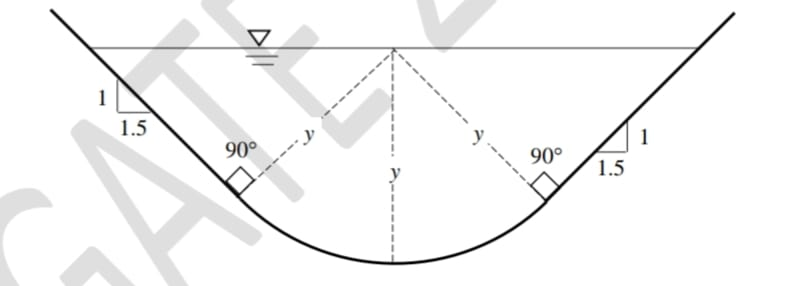
\includegraphics[width=0.7\columnwidth]{figs/1Q57.jpg}
        \caption{}
        \label{fig:q57}
    \end{figure}
    The normal depth of flow, $y$ \brak{\text{in meters}} for carrying a discharge of 20 m$^3$/s is \underline{\hspace{2cm}} \brak{\text{rounded off to 2 decimal places}}.
    
    \hfill{\brak{\text{GATE CE 2024}}}
    
    \item A spillway has unit discharge of 7.5 m$^3$/s/m. The flow depth at the downstream horizontal apron is 0.5 m. The tail water depth \brak{\text{in meters}} required to form a hydraulic jump is \underline{\hspace{2cm}} \brak{\text{rounded off to 2 decimal places}}.
    
    \hfill{\brak{\text{GATE CE 2024}}}
    
    \item A 5 m $\times$ 5 m closed tank of 10 m height contains water and oil, and is connected to an overhead water reservoir as shown in the figure \figref{fig:q59}. Use $\gamma_w = 10$ kN/m$^3$ and Specific gravity of oil = 0.8.
    \begin{figure}[H]
        \centering
        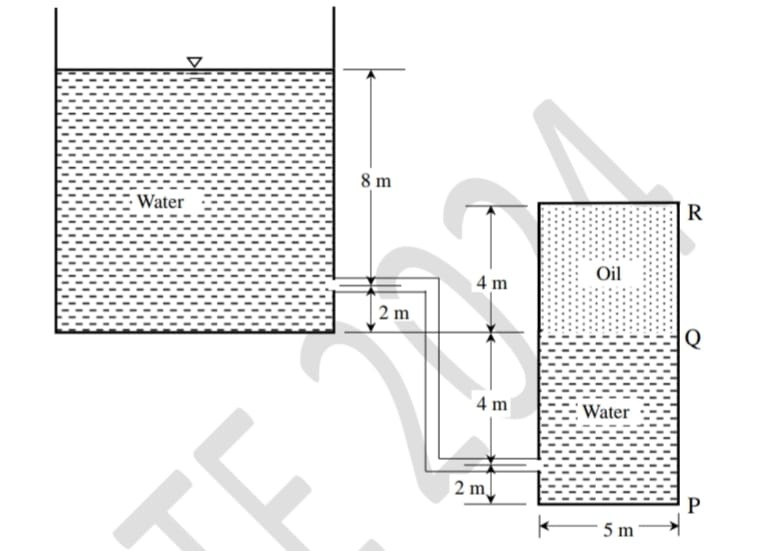
\includegraphics[width=0.7\columnwidth]{figs/1Q59.jpg}
        \caption{}
        \label{fig:q59}
    \end{figure}
    The total force \brak{\text{in kN}} due to pressure on the side PQR of the tank is \underline{\hspace{2cm}} \brak{\text{rounded off to the nearest integer}}.
    
    \hfill{\brak{\text{GATE CE 2024}}}
    
    \item Activated carbon is used to remove a pollutant from wastewater in a mixed batch reactor, which follows first-order reaction kinetics.
    At a reaction rate of 0.38 /day, the time \brak{\text{in days}} required to remove the pollutant by 95\% is \underline{\hspace{2cm}} \brak{\text{rounded off to 1 decimal place}}.
    
    \hfill{\brak{\text{GATE CE 2024}}}
    
    \item A water treatment plant treats 25 MLD water with a natural 
    alkalinity of 4.0 mg/L \brak{\text{as $CaCO_3$}}. It is estimated that,
    during coagulation of this water, 450 kg/day of calcium bicarbonate \brak{Ca\brak{HCO_3}_2} is required based on the alum dosage.
    Consider the atomic weights as: Ca-40, H-1, C-12, O-16.
    The quantity of pure quick lime, CaO \brak{\text{in kg}} required for this process per day is \underline{\hspace{2cm}} \brak{\text{rounded off to 2 decimal places}}.
    
    \hfill{\brak{\text{GATE CE 2024}}}
    
    \item The number of trains and their corresponding speeds for a curved Broad Gauge section with 437 m radius, are
    \begin{itemize}
        \item 20 trains travel at a speed of 40 km/hr
        \item 15 trains travel at a speed of 50 km/hr
        \item 12 trains travel at a speed of 60 km/hr
        \item 8 trains travel at a speed of 70 km/hr
        \item 3 trains travel at a speed of 80 km/hr
    \end{itemize}
    If the gauge \brak{\text{center-to-center distance between the rail heads}} is taken as 1750 mm, the required equilibrium cant \brak{\text{in mm}} will be \underline{\hspace{2cm}} \\
    \brak{\text{rounded off to the nearest integer}}.
    
    \hfill{\brak{\text{GATE CE 2024}}}
    
    \item The figure \figref{fig:q63} presents the trajectories of six vehicles within a time-space domain. The number in the parentheses represents unique identification of each vehicle.
    \begin{figure}[H]
        \centering
        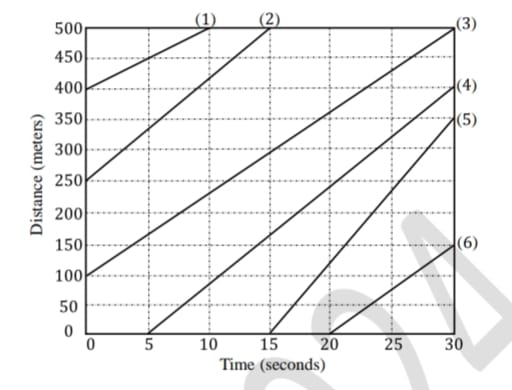
\includegraphics[width=0.7\columnwidth]{figs/1Q63.jpg}
        \caption{}
        \label{fig:q63}
    \end{figure}
    The mean speed \brak{\text{in km/hr}} of the vehicles in the entire time-space domain is \underline{\hspace{2cm}} \brak{\text{rounded off to the nearest integer}}.
    
    \hfill{\brak{\text{GATE CE 2024}}}
    
    \item The following data is obtained from an axle load survey at a site:
    
    Average rear axle load = 12000 kg\\
    Number of commercial vehicles = 800 per day
    
    The pavement at this site would be reconstructed over a period of 5 years from the date of survey. The design life of the reconstructed pavement is 15 years. Use the standard axle load as 8160 kg and the annual average vehicle growth rate as 4.0\%. Assume that Equivalent Wheel Load Factor \brak{EWLF} and Vehicle Damage Factor \brak{VDF} are equal.
    The cumulative standard axle \brak{\text{in msa}} for the pavement design is \underline{\hspace{2cm}} \brak{\text{rounded off to 2 decimal places}}.
    
    \hfill{\brak{\text{GATE CE 2024}}}
    
    \item A bird is resting on a point P at a height of 8 m above the Mean Sea Level \brak{MSL}. Upon hearing a loud noise, the bird flies parallel to the ground surface and reaches a point Q which is located at a height of 3 m above $MSL$. The ground surface has a falling gradient of 1 in 2. Ignoring the effects of curvature and refraction, the horizontal distance \brak{\text{in meters}} between points P and Q is \underline{\hspace{2cm}} \brak{\text{in integer}}.
    
    \hfill{\brak{\text{GATE CE 2024}}}

\end{enumerate}

\textbf{SESSION - 2}

\section*{General Aptitude \brak{GA}}
\textbf{Q.1 - Q.5 Carry ONE mark each}
\begin{enumerate}
    \item If '$\rightarrow$' denotes increasing order of intensity, then the meaning of the words
    \sbrak{\text{drizzle $\rightarrow$ rain $\rightarrow$ downpour}} is analogous to \sbrak{\text{ \underline{\hspace{2cm}} $\rightarrow$ quarrel $\rightarrow$ feud}}.
    Which one of the given options is appropriate to fill the blank?

    \hfill{\brak{\text{GATE CE 2024}}}
    \begin{enumerate}
        \begin{multicols}{4}
        \item bicker
        \item bog
        \item dither
        \item dodge
        \end{multicols}
    \end{enumerate}

    \item Statements:
    \begin{enumerate}
        \item All heroes are winners.
        \item All winners are lucky people.
    \end{enumerate}
    Inferences:
    \begin{enumerate}
        \item I. All lucky people are heroes.
        \item II. Some lucky people are heroes.
        \item III. Some winners are heroes.
    \end{enumerate}
    Which of the above inferences can be logically deduced from statements $1$ and $2$?

    \hfill{\brak{\text{GATE CE 2024}}}
    \begin{enumerate}
        \begin{multicols}{2}
        \item Only I and II
        \item Only II and III
        \item Only I and III
        \item Only III
        \end{multicols}
    \end{enumerate}

    \item A student was supposed to multiply a positive real number $p$ with another positive
    real number $q$. Instead, the student divided $p$ by $q$. If the percentage error in the
    student's answer is $80\%$, the value of $q$ is

    \hfill{\brak{\text{GATE CE 2024}}}
    \begin{enumerate}
        \begin{multicols}{4}
        \item $5$
        \item $\sqrt{2}$
        \item $2$
        \item $\sqrt{5}$
        \end{multicols}
    \end{enumerate}

    \item If the sum of the first $20$ consecutive positive odd numbers is divided by $20^2$, the
    result is

    \hfill{\brak{\text{GATE CE 2024}}}
    \begin{enumerate}
        \begin{multicols}{4}
        \item $1$
        \item $20$
        \item $2$
        \item $1/2$
        \end{multicols}
    \end{enumerate}

    \item The ratio of the number of girls to boys in class VIII is the same as the ratio of the
    number of boys to girls in class IX. The total number of students \brak{\text{boys and girls}} in
    classes VIII and IX is $450$ and $360$, respectively. If the number of girls in classes
    VIII and IX is the same, then the number of girls in each class is

    \hfill{\brak{\text{GATE CE 2024}}}
    \begin{enumerate}
        \begin{multicols}{4}
        \item $150$
        \item $200$
        \item $250$
        \item $175$
        \end{multicols}
    \end{enumerate}

    \textbf{Q.6 - Q.10 Carry ONE mark Each}
    \item In the given text, the blanks are numbered \brak{\text{i}}-\brak{\text{iv}}. Select the best match for
    all the blanks.\\
    Yoko Roi stands \underline{\hspace{1cm}} \brak{\text{i}} as an author for standing \underline{\hspace{1cm}} \brak{\text{ii}} as an honorary
    fellow, after she stood \underline{\hspace{1cm}} \brak{\text{iii}}  her writings that stand \underline{\hspace{1cm}} \brak{\text{iv}} the freedom of
    speech.
    
    \hfill{\brak{\text{GATE CE 2024}}}
    \begin{enumerate}
        \item \brak{\text{i}} out \brak{\text{ii}} down \brak{\text{iii}} in \brak{\text{iv}} for
        \item \brak{\text{i}} down \brak{\text{ii}} out \brak{\text{iii}} by \brak{\text{iv}} in
        \item \brak{\text{i}} down \brak{\text{ii}} out \brak{\text{iii}} for \brak{\text{iv}} in
        \item \brak{\text{i}} out \brak{\text{ii}} down \brak{\text{iii}} by \brak{\text{iv}} for
    \end{enumerate}

    \item Seven identical cylindrical chalk-sticks are fitted tightly in a cylindrical container.
    The figure \figref{fig:q7} below shows the arrangement of the chalk-sticks inside the cylinder.
    \begin{figure}[H]
        \centering
        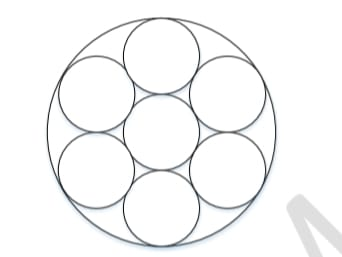
\includegraphics[width=0.7\columnwidth]{figs/2Q7.jpg}
        \caption{}
        \label{fig:q7}
    \end{figure}
    The length of the container is equal to the length of the chalk-sticks. The ratio of the occupied space to the empty space of the container is
    
    \hfill{\brak{\text{GATE CE 2024}}}
    \begin{enumerate}
        \begin{multicols}{4}
        \item $5/2$
        \item $7/2$
        \item $9/2$
        \item $3$
        \end{multicols}
    \end{enumerate}

    \item The plot \figref{fig:q8} below shows the relationship between the mortality risk of cardiovascular
    disease and the number of steps a person walks per day. Based on the data, which
    one of the following options is true?
    \begin{figure}[H]
        \centering
        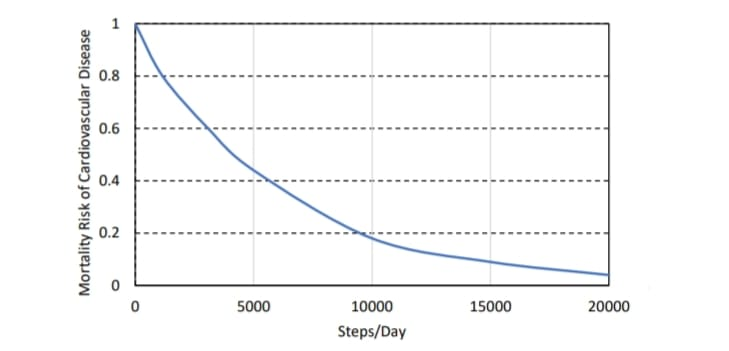
\includegraphics[width=0.7\columnwidth]{figs/2Q8.jpg}
        \caption{}
        \label{fig:q8}
    \end{figure}
    
    \hfill{\brak{\text{GATE CE 2024}}}
    \begin{enumerate}
        \item The risk reduction on increasing the steps/day from $0$ to $10000$ is less than the risk
        reduction on increasing the steps/day from $10000$ to $20000$.
        \item The risk reduction on increasing the steps/day from $0$ to $5000$ is less than the risk
        reduction on increasing the steps/day from $15000$ to $20000$.
        \item For any $5000$ increment in steps/day the largest risk reduction occurs on going from
        $0$ to $5000$.
        \item For any $5000$ increment in steps/day the largest risk reduction occurs on going from
        $15000$ to $20000$.
    \end{enumerate}

    \item Five cubes of identical size and another smaller cube are assembled as shown in
    Figure A \figref{fig:q9a}. If viewed from direction X, the planar image of the assembly appears as
    Figure B \figref{fig:q9b}.
    \begin{figure}[H]
        \centering
        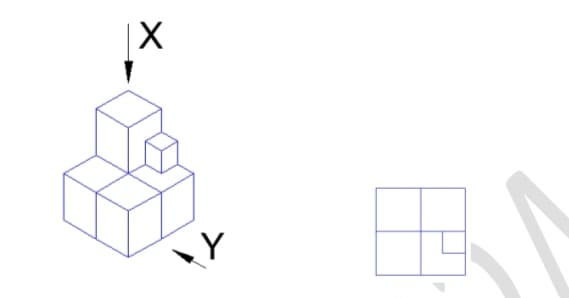
\includegraphics[width=0.7\columnwidth]{figs/2Q9.jpg}
        \caption{}
        \label{fig:q9a}
    \end{figure}
    
    If viewed from direction Y, the planar image of the assembly \brak{\text{Figure A}} will
    appear as
    
    \hfill{\brak{\text{GATE CE 2024}}}
    \begin{multicols}{2}
    \begin{enumerate}
    \item \begin{figure}[H]
        \centering
        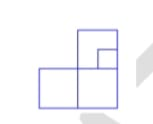
\includegraphics[width=0.5\columnwidth]{figs/2Q9a.jpg}
        \caption{}
        \label{fig:q9}
    \end{figure}
    \item \begin{figure}[H]
        \centering
        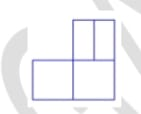
\includegraphics[width=0.5\columnwidth]{figs/2Q9b.jpg}
        \caption{}
        \label{fig:q9}
    \end{figure}
    \item \begin{figure}[H]
        \centering
        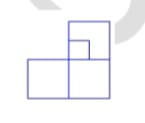
\includegraphics[width=0.5\columnwidth]{figs/2Q9c.jpg}
        \caption{}
        \label{fig:q9}
    \end{figure}
    \item \begin{figure}[H]
        \centering
        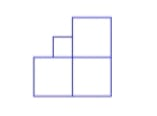
\includegraphics[width=0.5\columnwidth]{figs/2Q9d.jpg}
        \caption{}
        \label{fig:q9}
    \end{figure}
    \end{enumerate}
    \end{multicols}

    \item Visualize a cube that is held with one of the four body diagonals aligned to the vertical axis. Rotate the cube about this axis such that its view remains unchanged.
    The magnitude of the minimum angle of rotation is
    
    \hfill{\brak{\text{GATE CE 2024}}}
    \begin{enumerate}
        \begin{multicols}{4}
        \item $120\degree$
        \item $60\degree$
        \item $90\degree$
        \item $180\degree$
        \end{multicols}
    \end{enumerate}

    \item A partial differential equation
    \begin{align}
    \frac{\partial^2 T}{\partial x^2} + \frac{\partial^2 T}{\partial y^2} = 0
    \end{align}
    is defined for the two-dimensional field $T\colon T\brak{x, y}$, inside a planar square domain
    of size $2$ m $\times$ $2$ m. Three boundary edges of the square domain are maintained at
    value $T = 50$, whereas the fourth boundary edge is maintained at
    $T = 100$.
    The value of $T$ at the center of the domain is
    
    \hfill{\brak{\text{GATE CE 2024}}}
    \begin{enumerate}
        \begin{multicols}{4}
        \item $50.0$
        \item $62.5$
        \item $75.0$
        \item $87.5$
        \end{multicols}
    \end{enumerate}

    \item The statements P and Q are related to matrices $A$ and $B$, which are conformable for
    both addition and multiplication.
    \begin{align}
    P: \brak{A + B}^T = A^T + B^T
     \end{align}
     \begin{align}
    Q: \brak{AB}^T = A^T B^T
    \end{align}
    Which one of the following options is CORRECT?
    
    \hfill{\brak{\text{GATE CE 2024}}}
    \begin{enumerate}
        \begin{multicols}{2}
        \item P is TRUE and Q is FALSE
        \item Both P and Q are TRUE
        \item P is FALSE and Q is TRUE
        \item Both P and Q are FALSE
        \end{multicols}
    \end{enumerate}
    
    \item The second derivative of a function $f$ is computed using the fourth-order Central
    Divided Difference method with a step length $h$.
    The CORRECT expression for the second derivative is
    
    \hfill{\brak{\text{GATE CE 2024}}}
    \begin{enumerate}
        \item $\frac{1}{12h^2} \sbrak{-f_{i+2} + 16 f_{i+1} - 30 f_i + 16 f_{i-1} - f_{i-2}}$
        \item $\frac{1}{12h^2} \sbrak{f_{i+2} + 16 f_{i+1} - 30 f_i + 16 f_{i-1} - f_{i-2}}$
        \item $\frac{1}{12h^2} \sbrak{-f_{i+2} + 16 f_{i+1} - 30 f_i + 16 f_{i-1} + f_{i-2}}$
        \item $\frac{1}{12h^2} \sbrak{-f_{i+2} - 16 f_{i+1} + 30 f_i - 16 f_{i-1} - f_{i-2}}$
    \end{enumerate}

    \item The function 
    \begin{align}
    f\brak{x} = x^3 - 27x + 4, 1 \leq x \leq 6
    \end{align}
    has
    
    \hfill{\brak{\text{GATE CE 2024}}}
    \begin{enumerate}
        \begin{multicols}{2}
        \item Maxima point
        \item Minima point
        \item Saddle point
        \item Inflection point
        \end{multicols}
    \end{enumerate}

    \item Consider two Ordinary Differential Equations \brak{\text{ODEs}}:
    \begin{align}
    P\colon \quad \frac{dy}{dx} &= \frac{x^4+3x^2y^2+2y^4}{x^3y} \\
    Q\colon \quad \frac{dy}{dx} &= \frac{-y^2}{x^2}
    \end{align}
    Which one of the following options is CORRECT?
    
    \hfill{\brak{\text{GATE CE 2024}}}
    \begin{enumerate}
        \item P is a homogeneous ODE and Q is an exact ODE.
        \item P is a homogeneous ODE and Q is not an exact ODE.
        \item P is a nonhomogeneous ODE and Q is an exact ODE.
        \item P is a nonhomogeneous ODE and Q is not an exact ODE.
    \end{enumerate}

    \item A $3$ m long, horizontal, rigid, uniform beam PQ has negligible mass. The beam is
    subjected to a $3$ kN concentrated vertically downward force at $1$ m from P, as shown in the figure \figref{fig:q16}. The beam is resting on vertical linear springs at the ends P and Q. For
    the spring at the end P, the spring constant $K_p = 100$ kN/m.
    \begin{figure}[H]
        \centering
        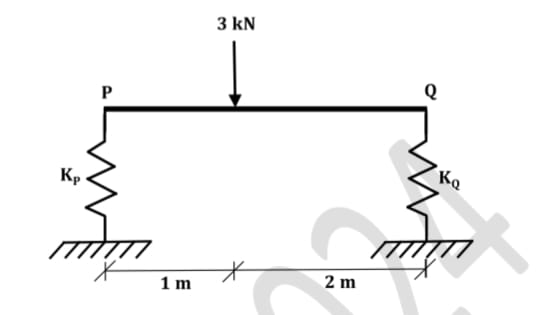
\includegraphics[width=0.7\columnwidth]{figs/2Q16.jpg}
        \caption{}
        \label{fig:q16}
    \end{figure}
    If the beam DOES NOT rotate under the application of the force and displaces only
    vertically, the value of the spring constant $K_q$ \brak{\text{in kN/m}} for the spring at the end Q is
    
    \hfill{\brak{\text{GATE CE 2024}}}
    \begin{enumerate}
        \begin{multicols}{4}
        \item $150$
        \item $100$
        \item $50$
        \item $200$
        \end{multicols}
    \end{enumerate}

    \item Consider the statements P and Q.
    
    P: In a Pure project organization, the project manager maintains complete authority
    and has maximum control over the project.
    
    Q: A Matrix organization structure facilitates quick response to changes, conflicts,
    and project needs.
    
    Which one of the following options is CORRECT?
    
    \hfill{\brak{\text{GATE CE 2024}}}
    \begin{enumerate}
        \begin{multicols}{2}
        \item Both P and Q are TRUE
        \item P is TRUE and Q is FALSE
        \item Both P and Q are FALSE
        \item P is FALSE and Q is TRUE
        \end{multicols}
    \end{enumerate}

    \item For a thin-walled section shown in the figure \figref{fig:q18}, points P, Q, and R are located on the
    major bending axis X - X of the section. Point Q is located on the web whereas point
    S is located at the intersection of the web and the top flange of the section.
    \begin{figure}[H]
        \centering
        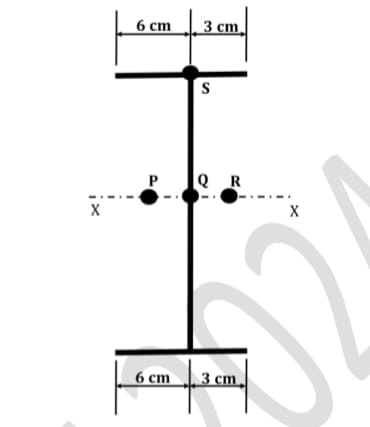
\includegraphics[width=0.7\columnwidth]{figs/2Q18.jpg}
        \caption{}
        \label{fig:q18}
    \end{figure}
    
    Qualitatively, the shear center of the section lies at
    
    \hfill{\brak{\text{GATE CE 2024}}}
    \begin{enumerate}
        \begin{multicols}{4}
        \item P
        \item Q
        \item R
        \item S
        \end{multicols}
    \end{enumerate}
    
    \item Consider the following data for a project of $300$ days duration.\\
    Budgeted Cost of Work Scheduled \brak{\text{BCWS}} = Rs. $200$
    
    Budgeted Cost of Work Performed \brak{\text{BCWP}} = Rs. $150$
    
    Actual Cost of Work Performed \brak{\text{ACWP}} = Rs. $190$
    
    The 'schedule variance' for the project is
    
    \hfill{\brak{\text{GATE CE 2024}}}
    \begin{enumerate}
        \begin{multicols}{2}
        \item \brak{\text{-}}Rs. $50$
        \item \brak{\text{-}}$50$ days
        \item \brak{\text{+}}Rs. $50$
        \item \brak{\text{+}}$50$ days
        \end{multicols}
    \end{enumerate}

    \item A simply supported, uniformly loaded, two-way slab panel is torsionally
    unrestrained. The effective span lengths along the short span \brak{\text{x}} and long span \brak{\text{y}}
    directions of the panel are $l_x$ and $l_y$, respectively. The design moments for the
    reinforcements along the $x$ and $y$ directions are $M_{ux}$ and $M_{uy}$, respectively. By using
    Rankine-Grashoff method, the ratio $M_{ux}/M_{uy}$ is proportional to
    
    \hfill{\brak{\text{GATE CE 2024}}}
    \begin{enumerate}
        \begin{multicols}{2}
        \item $l_x/l_y$
        \item $l_y/l_x$
        \item $\brak{l_x/l_y}^2$
        \item $\brak{l_y/l_x}^2$
        \end{multicols}
    \end{enumerate}
    
    \item The structural design method that DOES NOT take into account the safety factors
    on the design loads is
    
    \hfill{\brak{\text{GATE CE 2024}}}
    \begin{enumerate}
        \begin{multicols}{2}
        \item working stress method.
        \item load factor method.
        \item ultimate load method.
        \item limit state method.
        \end{multicols}
    \end{enumerate}
    
    \item The contact pressure distribution shown in the figure \figref{fig:q22} belongs to a
    \begin{figure}[H]
        \centering
        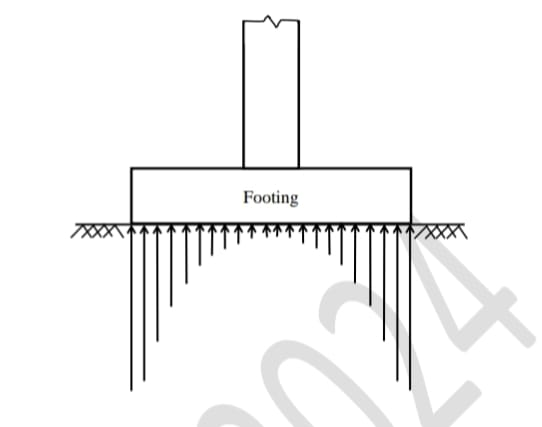
\includegraphics[width=0.7\columnwidth]{figs/2Q22.jpg}
        \caption{}
        \label{fig:q22}
    \end{figure}
    
    \hfill{\brak{\text{GATE CE 2024}}}
    \begin{enumerate}
        \item rigid footing resting on a cohesionless soil.
        \item rigid footing resting on a cohesive soil.
        \item flexible footing resting on a cohesionless soil.
        \item flexible footing resting on a cohesive soil.
    \end{enumerate}

    \item Which one of the following saturated fine-grained soils can attain a negative
    Skempton's pore pressure coefficient \brak{\text{A}}?
    
    \hfill{\brak{\text{GATE CE 2024}}}
    \begin{enumerate}
        \begin{multicols}{2}
        \item Quick clays
        \item Normally-consolidated clays
        \item Lightly-consolidated clays
        \item Over-consolidated clays
        \end{multicols}
    \end{enumerate}

    \item The following figure \figref{fig:q24} shows a plot between shear stress and velocity gradient for
    materials/fluids P, Q, R, S, and T.
    \begin{figure}[H]
        \centering
        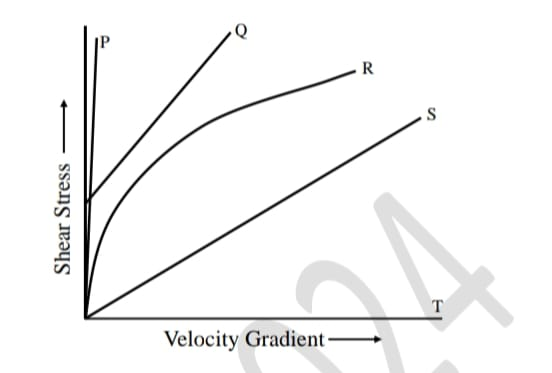
\includegraphics[width=0.7\columnwidth]{figs/2Q24.jpg}
        \caption{}
        \label{fig:q24}
    \end{figure}
    Which one of the following options is CORRECT?
    
    \hfill{\brak{\text{GATE CE 2024}}}
    \begin{enumerate}
        \item P $\rightarrow$ Ideal Fluid; Q $\rightarrow$ Ideal Bingham plastic
        R $\rightarrow$ Non-Newtonian fluid; S $\rightarrow$ Newtonian fluid
        \item P $\rightarrow$ Real solid; Q $\rightarrow$ Ideal Bingham plastic
        S $\rightarrow$ Newtonian fluid; T $\rightarrow$ Ideal Fluid
        \item P $\rightarrow$ Ideal Fluid; Q $\rightarrow$ Ideal Bingham plastic
        R $\rightarrow$ Non-Newtonian fluid; T $\rightarrow$ Real solid
        \item P $\rightarrow$ Real solid; Q $\rightarrow$ Newtonian fluid
        R $\rightarrow$ Ideal Bingham plastic; T $\rightarrow$ Ideal Fluid
    \end{enumerate}
    
    \item What is the CORRECT match between the air pollutants and treatment techniques
    given in the table?
    \begin{table}[H]
        \centering
        \begin{tabular}{|l|l|}
        \hline
        \textbf{Air pollutants} & \textbf{Treatment techniques} \\ \hline
        P - NO$_2$ & i - Flaring \\
        Q - SO$_2$ & ii - Cyclonic separator \\
        R - CO & iii - Lime scrubbing \\
        S - Particles & iv - NH$_3$ injection \\ \hline
        \end{tabular}
        \caption{}
        \label{tab:q25}
    \end{table}
    
    \hfill{\brak{\text{GATE CE 2024}}}
    \begin{enumerate}
        \begin{multicols}{2}
        \item P-i, Q-ii, R-iii, S-iv
        \item P-ii, Q-i, R-iv, S-iii
        \item P-ii, Q-iii, R-iv, S-i
        \item P-iv, Q-iii, R-i, S-ii
        \end{multicols}
    \end{enumerate}
    
    \item Which one of the following products is NOT obtained in anaerobic decomposition
    of glucose?
    
    \hfill{\brak{\text{GATE CE 2024}}}
    \begin{enumerate}
        \begin{multicols}{4}
        \item CO$_2$
        \item CH$_4$
        \item H$_2$S
        \item H$_2$O
        \end{multicols}
    \end{enumerate}

    \item The longitudinal sections of a runway have gradients as shown in the table.
    \begin{table}[H]
        \centering
        \begin{tabular}{|c|c|}
        \hline
        \textbf{End to end for sections of runway (m)} & \textbf{Gradient (\%)} \\ \hline
        $0$ to $200$ & $+1.0$ \\
        $200$ to $600$ & $-1.0$ \\
        $600$ to $1200$ & $+0.8$ \\
        $1200$ to $1600$ & $+0.2$ \\
        $1600$ to $2000$ & $-0.5$ \\ \hline
        \end{tabular}
        \caption{}
        \label{tab:q27}
    \end{table}
    Consider the reduced level \brak{\text{RL}} at the starting point of the runway as $100$ m.
    The effective gradient of the runway is
    
    \hfill{\brak{\text{GATE CE 2024}}}
    \begin{enumerate}
        \begin{multicols}{4}
        \item $0.02\%$
        \item $0.35\%$
        \item $0.28\%$
        \item $0.18\%$
        \end{multicols}
    \end{enumerate}
    
    \item In general, the outer edge is raised above the inner edge in horizontal curves for
    
    \hfill{\brak{\text{GATE CE 2024}}}
    \begin{enumerate}
        \item Highways, Railways, and Taxiways
        \item Highways and Railways only
        \item Railways and Taxiways only
        \item Highways only
    \end{enumerate}
    
    \item Various stresses in jointed plain concrete pavement with slab size of
    $3.5$ m $\times$ $4.5$ m are denoted as follows:
   \begin{itemize}
    \item Wheel load stress at interior = $S_{wl}^i$
    \item Wheel load stress at edge = $S_{wl}^e$
    \item Wheel load stress at corner = $S_{wl}^c$
    \item Warping stress at interior = $S_t^i$
    \item Warping stress at edge = $S_t^e$ 
    \item Warping stress at corner = $S_t^c$ 
    \item Frictional stress between slab and supporting layer = $S_f$
    \end{itemize}
    The critical stress combination in the concrete slab during a summer midnight is
    
    \hfill{\brak{\text{GATE CE 2024}}}
    \begin{enumerate}
        \item $S_{wl}^c + S_t^c$
        \item $S_{wl}^e + S_t^e + S_f$
        \item $S_{wl}^i + S_t^e - S_f$
        \item $S_{wl}^c + S_t^c + S_f$
    \end{enumerate}

    \item For a reconnaissance survey, it is necessary to obtain vertical aerial photographs of
    a terrain at an average scale of $1\colon13000$ using a camera. If the permissible flying
    height is assumed as $3000$ m above a datum and the average terrain elevation is
    $1050$ m above the datum, the required focal length \brak{\text{in mm}} of the camera is
    
    \hfill{\brak{\text{GATE CE 2024}}}
    \begin{enumerate}
        \begin{multicols}{4}
        \item $100$
        \item $150$
        \item $125$
        \item $200$
        \end{multicols}
    \end{enumerate}

    \item What is the CORRECT match between the survey instruments/parts of instruments
    shown in the table and the operations carried out with them?
    \begin{table}[H]
        \centering
        \begin{tabular}{|l|l|}
        \hline
        \textbf{Instruments/Parts of instruments} & \textbf{Operations} \\ \hline
        P - Bubble tube & i - Tacheometry \\
        Q - Plumb bob & ii - Minor movements \\
        R - Tangent screw & iii - Centering \\
        S - Stadia cross-wire & iv - Levelling \\ \hline
        \end{tabular}
        \caption{}
        \label{tab:q31}
    \end{table}

    \hfill{\brak{\text{GATE CE 2024}}}
    \begin{enumerate}
        \begin{multicols}{2}
        \item P-ii, Q-iii, R-iv, S-i
        \item P-iv, Q-iii, R-ii, S-i
        \item P-i, Q-iii, R-ii, S-iv
        \item P-iii, Q-iv, R-i, S-ii
        \end{multicols}
    \end{enumerate}
    
    \item To finalize the direction of a survey, four surveyors set up a theodolite at a station
    P and performed all the temporary adjustments. From the station P, each of the
    surveyors observed the bearing to a tower located at station Q with the same
    instrument without shifting it. The bearings observed by the surveyors are
    $30\degree 30' 00''$, $30\degree 29' 40''$, $30\degree 30' 20''$ and $30\degree 31' 20''$. Assuming that
    each measurement is taken with equal precision, the most probable value of the
    bearing is
    
    \hfill{\brak{\text{GATE CE 2024}}}
    \begin{enumerate}
        \begin{multicols}{2}
        \item $30\degree 29' 40''$
        \item $30\degree 30' 20''$
        \item $30\degree 30' 00''$
        \item $30\degree 31' 20''$
        \end{multicols}
    \end{enumerate}

    \item The steel angle section shown in the figure \figref{fig:q33} has elastic section modulus of
    $150.92 cm^3$ about the horizontal X - X axis, which passes through the centroid of
    the section.
    \begin{figure}[H]
        \centering
        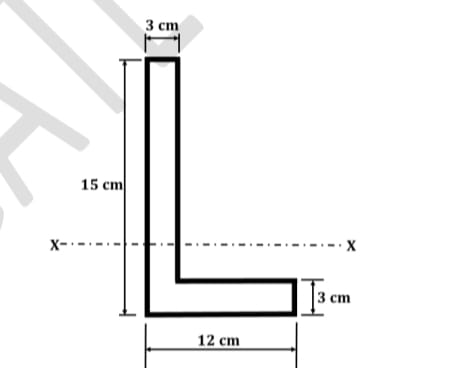
\includegraphics[width=0.7\columnwidth]{figs/2Q33.jpg}
        \caption{}
        \label{fig:q33}
    \end{figure}
    
    The shape factor of the section is \underline{\hspace{2cm}} \brak{\text{rounded off to 2 decimal places}}.
    
    \hfill{\brak{\text{GATE CE 2024}}}
    
    \item A reinforced concrete pile of $10$ m length and $0.7$ m diameter is embedded in a
    saturated pure clay with unit cohesion of $50$ kPa. If the adhesion factor is $0.5$, the
    net ultimate uplift pullout capacity \brak{\text{in kN}} of the pile is \underline{\hspace{2cm}}
    \brak{\text{rounded off to the nearest integer}}.
    
    \hfill{\brak{\text{GATE CE 2024}}}
    
    \item A $2$ m wide rectangular channel is carrying a discharge of $30 m^3/s$ at a bed slope of
    $1$ in $300$. Assuming the energy correction factor as $1.1$ and acceleration due to
    gravity as $10 m/s^2$, the critical depth of flow \brak{\text{in meters}} is \underline{\hspace{2cm}} \brak{\text{rounded
    off to 2 decimal places}}.
    
    \hfill{\brak{\text{GATE CE 2024}}}

\textbf{Q.36 - Q.65 Carry TWO marks Each}

    \item In a sample of $100$ heart patients, each patient has $80\%$ chance of having a heart
    attack without medicine X. It is clinically known that medicine X reduces the
    probability of having a heart attack by $50\%$. Medicine X is taken by $50$ of these $100$
    patients. The probability that a randomly selected patient, out of the $100$ patients,
    takes medicine X and has a heart attack is
    
    \hfill{\brak{\text{GATE CE 2024}}}
    \begin{enumerate}
        \begin{multicols}{4}
        \item $40\%$
        \item $60\%$
        \item $20\%$
        \item $30\%$
        \end{multicols}
    \end{enumerate}

    \item A linearly elastic beam of length $2l$ with flexural rigidity $EI$ has negligible mass.
    A massless spring with a spring constant $k$ and a rigid block of mass $m$ are attached
    to the beam as shown in the figure \figref{fig:q37}.
    \begin{figure}[H]
        \centering
        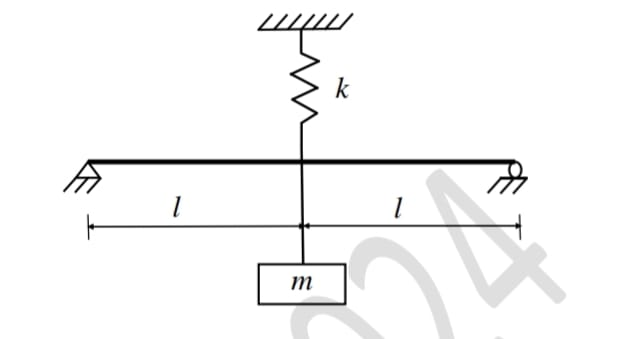
\includegraphics[width=0.7\columnwidth]{figs/2Q37.jpg}
        \caption{}
        \label{fig:q37}
    \end{figure}
    The natural frequency of this system is
    
    \hfill{\brak{\text{GATE CE 2024}}}
    \begin{enumerate}
        \item $\sqrt{\frac{kl^3 + 6EI}{ml^3}}$
        \item $\sqrt{\frac{kl^3 + 48EI}{ml^3}}$
        \item $\sqrt{\frac{6Elk}{(kl^3 + 6EI)m}}$
        \item $\sqrt{\frac{48Elk}{(kl^3 + 48EI)m}}$
    \end{enumerate}

    \item A critical activity in a project is estimated to take $15$ days to complete at a cost of Rs.
    $30,000$. The activity can be expedited to complete in $12$ days by spending a total
    amount of Rs. $54,000$. Consider the statements P and Q.
    
    P: It is economically advisable to complete the activity early by crashing, if the
    indirect cost of the project is Rs. $8,500$ per day.
    
    Q: It is economically advisable to complete the activity early by crashing, if the
    indirect cost of the project is Rs. $10,000$ per day.
    
    Which one of the following options is CORRECT?
    
    \hfill{\brak{\text{GATE CE 2024}}}
    \begin{enumerate}
        \begin{multicols}{2}
        \item Both P and Q are TRUE
        \item P is TRUE and Q is FALSE
        \item Both P and Q are FALSE
        \item P is FALSE and Q is TRUE
        \end{multicols}
    \end{enumerate}

    \item A homogeneous, prismatic, linearly elastic steel bar fixed at both the ends has a
    slenderness ratio \brak{\text{l/r}} of $105$, where l is the bar length and r is the radius of gyration.
    The coefficient of thermal expansion of steel is $12 \times 10^{-6} /\degree C$. Consider the effective
    length of the steel bar as $0.5l$ and neglect the self-weight of the bar.
    The differential increase in temperature \brak{\text{rounded off to the nearest integer}} at which
    the bar buckles is
    
    \hfill{\brak{\text{GATE CE 2024}}}
    \begin{enumerate}
        \begin{multicols}{2}
        \item $298 \degree C$
        \item $85 \degree C$
        \item $400 \degree C$
        \item $250 \degree C$
        \end{multicols}
    \end{enumerate}

    \item Consider the statements P and Q related to the analysis/design of retaining walls.
    
    P: When a rough retaining wall moves toward the backfill, the wall friction
    force/resistance mobilizes in upward direction along the wall.
    
    Q: Most of the earth pressure theories calculate the earth pressure due to surcharge
    by neglecting the actual distribution of stresses due to surcharge.
    
    Which one of the following options is CORRECT?
    
    \hfill{\brak{\text{GATE CE 2024}}}
    \begin{enumerate}
        \begin{multicols}{2}
        \item Both P and Q are TRUE
        \item P is TRUE and Q is FALSE
        \item Both P and Q are FALSE
        \item P is FALSE and Q is TRUE
        \end{multicols}
    \end{enumerate}
    
    \item A round-bottom triangular lined canal is to be laid at a slope of $1$ in $1500$, to carry
    a discharge of $25 m^3/s$. The side slopes of the canal cross-section are to be kept at
    $1.25H:1V$. If Manning's roughness coefficient is $0.013$, the flow depth
    \brak{\text{in meters}} will be in the range of
    
    \hfill{\brak{\text{GATE CE 2024}}}
    \begin{enumerate}
        \begin{multicols}{2}
        \item $2.39$ to $2.42$
        \item $1.94$ to $1.97$
        \item $2.24$ to $2.27$
        \item $2.61$ to $2.64$
        \end{multicols}
    \end{enumerate}

    \item A hypothetical multimedia filter, consisting of anthracite particles\\ \brak{\text{specific gravity: 1.50}}, silica sand \brak{\text{specific gravity: 2.60}}, and ilmenite sand \brak{\text{specific gravity: 4.20}},
    is to be designed for treating water/wastewater. After backwashing, the particles
    should settle forming three layers: coarse anthracite particles at the top of the bed,
    silica sand in the middle, and small ilmenite sand particles at the bottom of the bed.
    
    Assume
    \begin{enumerate}
        \item[\brak{\text{i}}] Slow discrete settling \brak{\text{Stoke's law is applicable}}
        \item[\brak{\text{ii}}] All particles are spherical
        \item[\brak{\text{iii}}] Diameter of silica sand particles is $0.20$ mm
    \end{enumerate}
    The CORRECT option fulfilling the diameter requirements for this filter media is
    
    \hfill{\brak{\text{GATE CE 2024}}}
    \begin{enumerate}
        \item diameter of anthracite particles is slightly less than $0.35$ mm and diameter of ilmenite
        particles is slightly greater than $0.141$ mm.
        \item diameter of anthracite particles is slightly greater than $0.35$ mm and diameter of
        ilmenite particles is slightly less than $0.141$ mm.
        \item diameter of anthracite particles is slightly less than $0.64$ mm and diameter of ilmenite
        particles is slightly less than $0.10$ mm.
        \item diameter of anthracite particles is slightly greater than $0.64$ mm and diameter of
        ilmenite particles is slightly less than $0.10$ mm.
    \end{enumerate}

    \item The consolidated data of a spot speed study for a certain stretch of a highway is given
    in the table.
    \begin{table}[H]
        \centering
        \begin{tabular}{|c|c|}
        \hline
        \textbf{Speed range (kmph)} & \textbf{Number of observations} \\ \hline
        $0-10$ & $7$ \\
        $10-20$ & $31$ \\
        $20-30$ & $76$ \\
        $30-40$ & $129$ \\
        $40-50$ & $104$ \\
        $50-60$ & $78$ \\
        $60-70$ & $29$ \\
        $70-80$ & $24$ \\
        $80-90$ & $13$ \\
        $90-100$ & $9$ \\ \hline
        \end{tabular}
        \caption{}
        \label{tab:q43}
    \end{table}
    The "upper speed limit" \brak{\text{in kmph}} for the traffic sign is
    
    \hfill{\brak{\text{GATE CE 2024}}}
    \begin{enumerate}
        \begin{multicols}{4}
        \item $50$
        \item $55$
        \item $65$
        \item $70$
        \end{multicols}
    \end{enumerate}
    
    \item Three vectors $\vec{p}$, $\vec{q}$, and $\vec{r}$ are given as
    \begin{align}
        \vec{p} &= \hat{i} + \hat{j} + \hat{k} \\
        \vec{q} &= \hat{i} + 2\hat{j} + 3\hat{k} \\
        \vec{r} &= 2\hat{i} + 3\hat{j} + 4\hat{k}
    \end{align}
    Which of the following is/are CORRECT?
    
    \hfill{\brak{\text{GATE CE 2024}}}
    \begin{enumerate}
        \item $\vec{p} \times \brak{\vec{q} \times \vec{r}} + \vec{q} \times \brak{\vec{r} \times \vec{p}} + \vec{r} \times \brak{\vec{p} \times \vec{q}} = \vec{0}$
        \item $\vec{p} \times \brak{\vec{q} \times \vec{r}} = \brak{\vec{p} \cdot \vec{r}}\vec{q} - \brak{\vec{p} \cdot \vec{q}}\vec{r}$
        \item $\vec{p} \times \brak{\vec{q} \times \vec{r}} = \brak{\vec{p} \times \vec{q}} \times \vec{r}$
        \item $\vec{r} \cdot \brak{\vec{p} \times \vec{q}} = \brak{\vec{q} \times \vec{p}} \cdot \vec{r}$
    \end{enumerate}

    \item Consider the statements P, Q, and R.
    
    P: Compacted fine-grained soils with flocculated structure have isotropic
    permeability.
    
    Q: Phreatic surface/line is the line along which the pore water pressure is always
    maximum.
    
    R: The piping phenomenon occurring below the dam foundation is typically known
    as blowout piping.
    
    Which of the following option is/are CORRECT?
    
    \hfill{\brak{\text{GATE CE 2024}}}
    \begin{enumerate}
        \begin{multicols}{2}
        \item Both P and R are TRUE
        \item P is FALSE and Q is TRUE
        \item P is TRUE and R is FALSE
        \item Both Q and R are FALSE
        \end{multicols}
    \end{enumerate}

    \item In the context of pavement material characterization, the CORRECT statement is/are
    \hfill{\brak{\text{GATE CE 2024}}}
    \begin{enumerate}
        \item The load penetration curve of CBR test may need origin correction due to the
        non-vertical penetrating plunger of the loading machine.
        \item The toughness and hardness of road aggregates are determined by Los Angeles
        abrasion test and aggregate impact test, respectively.
        \item Grading of normal (unmodified) bitumen binders is done based on viscosity test
        results.
        \item In compacted bituminous mix, Voids in the Mineral Aggregate \brak{\text{VMA}} is equal to
        the sum of total volume of air voids \brak{V_a} and total volume of bitumen \brak{V_b}.
    \end{enumerate}

    \item The expression for computing the effective interest rate \brak{i_{eff}} using continuous
    compounding for a nominal interest rate of $5\%$ is
    \begin{align}
    i_{eff} = \lim_{m \to \infty} \brak{1 + \frac{0.05}{m}}^m - 1
    \end{align}
    The effective interest rate \brak{\text{in percentage}} is \underline{\hspace{2cm}} \\
    \brak{\text{rounded off to 2 decimal places}}.
    
    \hfill{\brak{\text{GATE CE 2024}}}

    \item Consider two matrices $A = \myvec{2 & 1 & 4 \\ 1 & 0 & 3}$ and $B = \myvec{-1 & 0 \\ 2 & 3 \\ 1 & 4}$.
    The determinant of the matrix $AB$ is \underline{\hspace{2cm}} \brak{\text{in integer}}.
    
    \hfill{\brak{\text{GATE CE 2024}}}

    \item For the $6$ m long horizontal cantilever beam PQR shown in the figure \figref{fig:q49}, Q is the mid-
    point. Segment PQ of the beam has flexural rigidity $EI = 2 \times 10^5 kN. m^2$
    whereas the segment QR has infinite flexural rigidity. Segment QR is subjected to
    uniformly distributed, vertically downward load of $5$ kN/m.
    \begin{figure}[H]
        \centering
        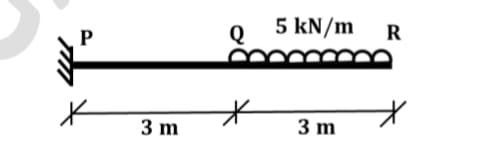
\includegraphics[width=0.7\columnwidth]{figs/2Q49.jpg}
        \caption{}
        \label{fig:q49}
    \end{figure}
    
    The magnitude of the vertical displacement \brak{\text{in mm}} at point Q is \underline{\hspace{2cm}} \brak{\text{rounded
    off to 3 decimal places}}.
    
    \hfill{\brak{\text{GATE CE 2024}}}

    \item The horizontal beam PQRS shown in the figure \figref{fig:q50} has a fixed support at point P, an
    internal hinge at point Q, and a pin support at point R. A concentrated vertically
    downward load \brak{\text{V}} of $10$ kN can act at any point over the entire length of the beam.
    \begin{figure}[H]
        \centering
        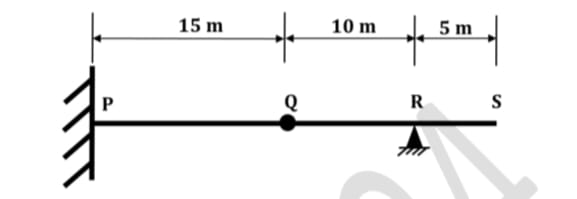
\includegraphics[width=0.7\columnwidth]{figs/2Q50.jpg}
        \caption{}
        \label{fig:q50}
    \end{figure}    
    The maximum magnitude of the moment reaction \brak{\text{in kN.m}} that can act at the
    support P due to V is \underline{\hspace{2cm}} \brak{\text{in integer}}.
    
    \hfill{\brak{\text{GATE CE 2024}}}

    \item A concrete column section of size $300$ mm $\times$ $500$ mm as shown in the figure \figref{fig:q51} is
    subjected to both axial compression and bending along the major axis. The depth of
    the neutral axis \brak{X_u} is $1.1$ times the depth of the column, as shown.
    \begin{figure}[H]
        \centering
        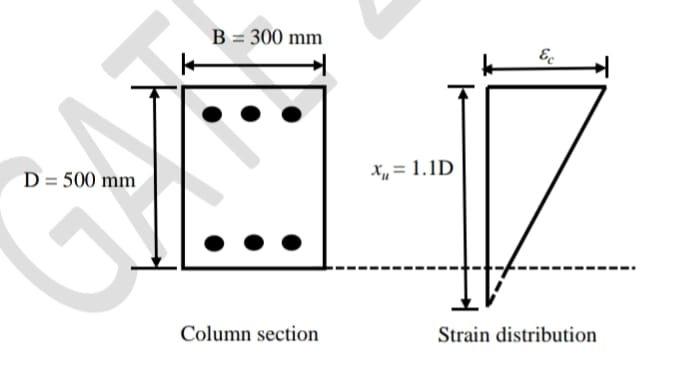
\includegraphics[width=0.7\columnwidth]{figs/2Q51.jpg}
        \caption{}
        \label{fig:q51}
    \end{figure}
    
    The maximum compressive strain \brak{\epsilon_c} at highly compressive extreme fiber in
    concrete, where there is no tension in the section, is \underline{\hspace{2cm}} $\times 10^{-3}$
    \brak{\text{rounded off to 2 decimal places}}.
    
    \hfill{\brak{\text{GATE CE 2024}}}

    \item The table shows the activities and their durations and dependencies in a project.
    \begin{table}[H]
        \centering
        \begin{tabular}{|c|c|c|}
        \hline
        \textbf{Activity} & \textbf{Duration (Days)} & \textbf{Depends on} \\ \hline
        A & $8$ & - \\
        B & $4$ & A \\
        C & $4$ & B \\
        D & $4$ & C, L \\
        F & $4$ & A \\
        G & $4$ & F \\
        H & $6$ & G, L \\
        K & $10$ & A \\
        L & $6$ & F, K \\ \hline
        \end{tabular}
        \caption{}
        \label{tab:q52}
    \end{table}
    The total duration \brak{\text{in days}} of the project is \underline{\hspace{2cm}} \brak{\text{in integer}}.
    
    \hfill{\brak{\text{GATE CE 2024}}}

    \item A homogeneous earth dam has a maximum water head difference of $15$ m between
    the upstream and downstream sides. A flownet was drawn with the number of
    potential drops as $10$ and the average length of the element as $3$ m. Specific gravity
    of the soil is $2.65$. For a factor of safety of $2.0$ against piping failure, void ratio of
    the soil is \underline{\hspace{2cm}} \\
    \brak{\text{rounded off to 2 decimal places}}.
    
    \hfill{\brak{\text{GATE CE 2024}}}
    
    \item The in-situ percentage of voids of a sand deposit is $50\%$. The maximum and
    minimum densities of sand determined from the laboratory tests are $1.8 g/cm^3$ and
    $1.3 g/cm^3$, respectively. Assume the specific gravity of sand as $2.7$.
    The relative density index of the in-situ sand is \underline{\hspace{2cm}} \\ \brak{\text{rounded off to 2
    decimal places}}.
    
    \hfill{\brak{\text{GATE CE 2024}}}

    \item A drained triaxial test was conducted on a saturated sand specimen using a
    stress-path triaxial testing system. The specimen failed when the axial stress reached
    a value of $100 kN/m^2$ from an initial confining pressure of $300 kN/m^2$.
    The angle of shearing plane \brak{\text{in degrees}} with respect to horizontal is
    \underline{\hspace{2cm}} \brak{\text{rounded off to the nearest integer}}.
    
    \hfill{\brak{\text{GATE CE 2024}}}
    
    \item A storm with a recorded precipitation of $11.0$ cm, as shown in the table, produced a
    direct run-off of $6.0$ cm.
    \begin{table}[H]
        \centering
        \begin{tabular}{|c|c|c|c|c|c|c|c|c|}
        \hline
        \textbf{Time from start (hours)} & $1$ & $2$ & $3$ & $4$ & $5$ & $6$ & $7$ & $8$ \\ \hline
        \textbf{Recorded cumulative} & & & & & & & & \\
        \textbf{precipitation (cm)} & $0.5$ & $1.5$ & $3.1$ & $5.5$ & $7.3$ & $8.9$ & $10.2$ & $11.0$ \\ \hline
        \end{tabular}
        \caption{}
        \label{tab:q56}
    \end{table}
    The $\o$-index of this storm is \underline{\hspace{2cm}} cm/hr \brak{\text{rounded off to 2 decimal places}}.
    
    \hfill{\brak{\text{GATE CE 2024}}}
    
    \item A $500$ m long water distribution pipeline P with diameter $1.0$ m, is used to convey
    $0.1 m^3/s$ of flow. A new pipeline Q, with the same length and flow rate, is to replace
    P. The friction factors for P and Q are $0.04$ and $0.01$, respectively. The diameter of
    the pipeline Q \brak{\text{in meters}} is \underline{\hspace{2cm}} \brak{\text{rounded off to 2 decimal places}}.
    
    \hfill{\brak{\text{GATE CE 2024}}}
    
    \item A $2$ m $\times$ $1.5$ m tank of $6$ m height is provided with a $100$ mm diameter orifice at the
    center of its base. The orifice is plugged and the tank is filled up to $5$ m height.
    Consider the average value of discharge coefficient as $0.6$ and acceleration due to
    gravity \brak{\text{g}} as $10 m/s^2$. After unplugging the orifice, the time \brak{\text{in seconds}} taken for
    the water level to drop from $5$ m to $3.5$ m under free discharge condition is
    \underline{\hspace{2cm}} \brak{\text{rounded off to 2 decimal places}}.
    
    \hfill{\brak{\text{GATE CE 2024}}}
    
    \item A rectangular channel is $4.0$ m wide and carries a discharge of $2.0 m^3/s$ with a depth
    of $0.4$ m. The channel transitions to a maximum width contraction at a downstream
    location, without influencing the upstream flow conditions. The width \brak{\text{in meters}} at
    the maximum contraction is \underline{\hspace{2cm}} \brak{\text{rounded off to 2 decimal places}}.
    
    \hfill{\brak{\text{GATE CE 2024}}}
    
    \item A circular settling tank is to be designed for primary treatment of sewage at a flow
    rate of $10$ million liters/day. Assume a detention period of $2.0$ hours and surface
    loading rate of $40000$ liters/m$^2$/day. The height \brak{\text{in meters}} of the water column in
    the tank is \underline{\hspace{2cm}} \brak{\text{rounded off to 2 decimal places}}.
    
    \hfill{\brak{\text{GATE CE 2024}}}

    \item An organic waste is represented as C$_{240}$O$_{200}$H$_{180}$N$_5$S.\\
    \brak{\text{Atomic weights: S-32, H-1, C-12, O-16, N-14}}.
    Assume complete conversion of S to SO$_2$ while burning.
    SO$_2$ generated \brak{\text{in grams}} per kg of this waste is \underline{\hspace{2cm}}
    \brak{\text{rounded off to 1 decimal place}}.
    
    \hfill{\brak{\text{GATE CE 2024}}}
    
    \item A horizontal curve of radius $1080$ m \brak{\text{with transition curves on either side}} in a Broad
    Gauge railway track is designed and constructed for an equilibrium speed of
    $70$ kmph. However, a few years after construction, the Railway Authorities decided
    to run express trains on this track. The maximum allowable cant deficiency is
    $10$ cm.
    The maximum restricted speed \brak{\text{in kmph}} of the express trains running on this track
    is \underline{\hspace{2cm}} \\ \brak{\text{rounded off to the nearest integer}}.
    
    \hfill{\brak{\text{GATE CE 2024}}}
    
    \item A vertical summit curve on a freight corridor is formed at the intersection of two
    gradients, $+3.0\%$ and $-5.0\%$.
    
    Assume the following:
    \begin{itemize}
    \item Only large-sized trucks are allowed on this corridor
    
    \item Design speed = $80$ kmph
    
    \item Eye height of truck drivers above the road surface = $2.30$ m
    
    \item Height of object above the road surface for which trucks need to stop = $0.35$ m
    
    \item Total reaction time of the truck drivers = $2.0$ s
    
    \item Coefficient of longitudinal friction of the road = $0.36$
    
    \item Stopping sight distance gets compensated on the gradient
    \end{itemize}
    The design length of the summit curve \brak{\text{in meters}} to accommodate the stopping sight
    distance is \underline{\hspace{2cm}} \brak{\text{rounded off to 2 decimal places}}.
    
    \hfill{\brak{\text{GATE CE 2024}}}
    
    \item A child walks on a level surface from point P to point Q at a bearing of $30\degree$, from
    point Q to point R at a bearing of $90\degree$ and then directly returns to the starting point P
    at a bearing of $240\degree$. The straight-line paths PQ and QR are $4$ m each. Assuming that
    all bearings are measured from the magnetic north in degrees, the straight-line path
    length RP \brak{\text{in meters}} is \underline{\hspace{2cm}} \brak{\text{rounded off to the nearest integer}}.
    
    \hfill{\brak{\text{GATE CE 2024}}}
    
    \item Differential levelling is carried out from point $P$ \brak{\text{BM: +200.000 m}} to point R.
    The readings taken are given in the table.
    \begin{table}[H]
        \centering
        \begin{tabular}{|c|c|c|c|}
        \hline
        & \multicolumn{2}{c|}{\textbf{Staff readings (m)}} & \\ \cline{2-3}
        \textbf{Points} & \textbf{Back Sight} & \textbf{Fore Sight} & \textbf{Remarks} \\ \hline
        P & \brak{\text{-}}$2.050$ & & BM: +$200.000$ m \\
        Q & $1.050$ & $0.950$ & Q is a change point \\
        R & & \brak{\text{-}}$1.655$ & \\ \hline
        \end{tabular}
        \caption{}
        \label{tab:q65}
    \end{table}
    Reduced Level \brak{\text{in meters}} of the point R is \underline{\hspace{2cm}} \\ \brak{\text{rounded off to 3 decimal places}}.
    
    \hfill{\brak{\text{GATE CE 2024}}}

\end{enumerate}

\end{document}
